% Options for packages loaded elsewhere
\PassOptionsToPackage{unicode}{hyperref}
\PassOptionsToPackage{hyphens}{url}
%
\documentclass[
]{article}
\usepackage{lmodern}
\usepackage{amssymb,amsmath}
\usepackage{ifxetex,ifluatex}
\ifnum 0\ifxetex 1\fi\ifluatex 1\fi=0 % if pdftex
  \usepackage[T1]{fontenc}
  \usepackage[utf8]{inputenc}
  \usepackage{textcomp} % provide euro and other symbols
\else % if luatex or xetex
  \usepackage{unicode-math}
  \defaultfontfeatures{Scale=MatchLowercase}
  \defaultfontfeatures[\rmfamily]{Ligatures=TeX,Scale=1}
\fi
% Use upquote if available, for straight quotes in verbatim environments
\IfFileExists{upquote.sty}{\usepackage{upquote}}{}
\IfFileExists{microtype.sty}{% use microtype if available
  \usepackage[]{microtype}
  \UseMicrotypeSet[protrusion]{basicmath} % disable protrusion for tt fonts
}{}
\makeatletter
\@ifundefined{KOMAClassName}{% if non-KOMA class
  \IfFileExists{parskip.sty}{%
    \usepackage{parskip}
  }{% else
    \setlength{\parindent}{0pt}
    \setlength{\parskip}{6pt plus 2pt minus 1pt}}
}{% if KOMA class
  \KOMAoptions{parskip=half}}
\makeatother
\usepackage{xcolor}
\IfFileExists{xurl.sty}{\usepackage{xurl}}{} % add URL line breaks if available
\IfFileExists{bookmark.sty}{\usepackage{bookmark}}{\usepackage{hyperref}}
\hypersetup{
  pdftitle={Statistical Literature and Problems},
  hidelinks,
  pdfcreator={LaTeX via pandoc}}
\urlstyle{same} % disable monospaced font for URLs
\usepackage[margin=1in]{geometry}
\usepackage{color}
\usepackage{fancyvrb}
\newcommand{\VerbBar}{|}
\newcommand{\VERB}{\Verb[commandchars=\\\{\}]}
\DefineVerbatimEnvironment{Highlighting}{Verbatim}{commandchars=\\\{\}}
% Add ',fontsize=\small' for more characters per line
\usepackage{framed}
\definecolor{shadecolor}{RGB}{248,248,248}
\newenvironment{Shaded}{\begin{snugshade}}{\end{snugshade}}
\newcommand{\AlertTok}[1]{\textcolor[rgb]{0.94,0.16,0.16}{#1}}
\newcommand{\AnnotationTok}[1]{\textcolor[rgb]{0.56,0.35,0.01}{\textbf{\textit{#1}}}}
\newcommand{\AttributeTok}[1]{\textcolor[rgb]{0.77,0.63,0.00}{#1}}
\newcommand{\BaseNTok}[1]{\textcolor[rgb]{0.00,0.00,0.81}{#1}}
\newcommand{\BuiltInTok}[1]{#1}
\newcommand{\CharTok}[1]{\textcolor[rgb]{0.31,0.60,0.02}{#1}}
\newcommand{\CommentTok}[1]{\textcolor[rgb]{0.56,0.35,0.01}{\textit{#1}}}
\newcommand{\CommentVarTok}[1]{\textcolor[rgb]{0.56,0.35,0.01}{\textbf{\textit{#1}}}}
\newcommand{\ConstantTok}[1]{\textcolor[rgb]{0.00,0.00,0.00}{#1}}
\newcommand{\ControlFlowTok}[1]{\textcolor[rgb]{0.13,0.29,0.53}{\textbf{#1}}}
\newcommand{\DataTypeTok}[1]{\textcolor[rgb]{0.13,0.29,0.53}{#1}}
\newcommand{\DecValTok}[1]{\textcolor[rgb]{0.00,0.00,0.81}{#1}}
\newcommand{\DocumentationTok}[1]{\textcolor[rgb]{0.56,0.35,0.01}{\textbf{\textit{#1}}}}
\newcommand{\ErrorTok}[1]{\textcolor[rgb]{0.64,0.00,0.00}{\textbf{#1}}}
\newcommand{\ExtensionTok}[1]{#1}
\newcommand{\FloatTok}[1]{\textcolor[rgb]{0.00,0.00,0.81}{#1}}
\newcommand{\FunctionTok}[1]{\textcolor[rgb]{0.00,0.00,0.00}{#1}}
\newcommand{\ImportTok}[1]{#1}
\newcommand{\InformationTok}[1]{\textcolor[rgb]{0.56,0.35,0.01}{\textbf{\textit{#1}}}}
\newcommand{\KeywordTok}[1]{\textcolor[rgb]{0.13,0.29,0.53}{\textbf{#1}}}
\newcommand{\NormalTok}[1]{#1}
\newcommand{\OperatorTok}[1]{\textcolor[rgb]{0.81,0.36,0.00}{\textbf{#1}}}
\newcommand{\OtherTok}[1]{\textcolor[rgb]{0.56,0.35,0.01}{#1}}
\newcommand{\PreprocessorTok}[1]{\textcolor[rgb]{0.56,0.35,0.01}{\textit{#1}}}
\newcommand{\RegionMarkerTok}[1]{#1}
\newcommand{\SpecialCharTok}[1]{\textcolor[rgb]{0.00,0.00,0.00}{#1}}
\newcommand{\SpecialStringTok}[1]{\textcolor[rgb]{0.31,0.60,0.02}{#1}}
\newcommand{\StringTok}[1]{\textcolor[rgb]{0.31,0.60,0.02}{#1}}
\newcommand{\VariableTok}[1]{\textcolor[rgb]{0.00,0.00,0.00}{#1}}
\newcommand{\VerbatimStringTok}[1]{\textcolor[rgb]{0.31,0.60,0.02}{#1}}
\newcommand{\WarningTok}[1]{\textcolor[rgb]{0.56,0.35,0.01}{\textbf{\textit{#1}}}}
\usepackage{longtable,booktabs}
% Correct order of tables after \paragraph or \subparagraph
\usepackage{etoolbox}
\makeatletter
\patchcmd\longtable{\par}{\if@noskipsec\mbox{}\fi\par}{}{}
\makeatother
% Allow footnotes in longtable head/foot
\IfFileExists{footnotehyper.sty}{\usepackage{footnotehyper}}{\usepackage{footnote}}
\makesavenoteenv{longtable}
\usepackage{graphicx,grffile}
\makeatletter
\def\maxwidth{\ifdim\Gin@nat@width>\linewidth\linewidth\else\Gin@nat@width\fi}
\def\maxheight{\ifdim\Gin@nat@height>\textheight\textheight\else\Gin@nat@height\fi}
\makeatother
% Scale images if necessary, so that they will not overflow the page
% margins by default, and it is still possible to overwrite the defaults
% using explicit options in \includegraphics[width, height, ...]{}
\setkeys{Gin}{width=\maxwidth,height=\maxheight,keepaspectratio}
% Set default figure placement to htbp
\makeatletter
\def\fps@figure{htbp}
\makeatother
\setlength{\emergencystretch}{3em} % prevent overfull lines
\providecommand{\tightlist}{%
  \setlength{\itemsep}{0pt}\setlength{\parskip}{0pt}}
\setcounter{secnumdepth}{-\maxdimen} % remove section numbering
\usepackage{amssymb}
\usepackage{amsmath}
\usepackage{booktabs}
\usepackage{longtable}
\usepackage{array}
\usepackage{multirow}
\usepackage{wrapfig}
\usepackage{float}
\usepackage{colortbl}
\usepackage{pdflscape}
\usepackage{tabu}
\usepackage{threeparttable}
\usepackage{threeparttablex}
\usepackage[normalem]{ulem}
\usepackage{makecell}
\usepackage{xcolor}

\title{Statistical Literature and Problems}
\usepackage{etoolbox}
\makeatletter
\providecommand{\subtitle}[1]{% add subtitle to \maketitle
  \apptocmd{\@title}{\par {\large #1 \par}}{}{}
}
\makeatother
\subtitle{STAT 501}
\author{}
\date{\vspace{-2.5em}15 July, 2020}

\begin{document}
\maketitle

\hypertarget{section}{%
\section{}\label{section}}

\hypertarget{albert-chib-1993}{%
\subsection{(Albert \& Chib, 1993)}\label{albert-chib-1993}}

James H. Albert \& Siddhartha Chib (1993) Bayesian Analysis of Binary
and Polychotomous Response Data, Journal of the American Statistical
Association, 88:422, 669-679,
\href{https://doi.org/10.1080/01621459.1993.10476321}{DOI:
10.1080/01621459.1993.10476321}

\hypertarget{introduction}{%
\subsubsection{1 Introduction}\label{introduction}}

\(Y_1,..,Y_n\sim Bern(p_i)\). \(\beta_{k\times1}\) unknown vector of
parameters. \(X_i^T=(X_{i1},..,X_{ik})\) known covariates.

\(p_i=H(\mathbf{x}_i^T\boldsymbol{\beta})\). \(H(\cdot)\) is a known CDF
with linear structure \(\mathbf{x}_i^T\boldsymbol{\beta}\)

If \(H(\cdot)\) is standard normal CDF, it obtains the probit model,

if \(H(\cdot)\) is logistic CDF, it obtains the logit model.

\(\pi(\boldsymbol{\beta})\) is the prior density.

\(\pi(\boldsymbol{\beta}|data) = \frac{\pi(\boldsymbol{\beta})\prod_{i=1}^{k}H (\mathbf{x}_i^T\boldsymbol{\beta})^{y_i}(1-H(\mathbf{x}_i^T\boldsymbol{\beta}))^{1-y_i}}{\int\pi(\boldsymbol{\beta})\prod_{i=1}^{k}H (\mathbf{x}_i^T\boldsymbol{\beta})^{y_i}(1-H(\mathbf{x}_i^T\boldsymbol{\beta}))^{1-y_i}d\boldsymbol{\beta}}\)
is intractable.

For small number of parameter, a Bayesian approach summarized the
posterior using numerical integration.

For large models (k large), posterior moments by Monte Carlo integration
with a
\texttt{multivariate\ Student\textquotesingle{}s\ t\ importance\ function}.

This is a simulation-based approach for computing the exact posterior
distribution of \(\beta\).

The key idea is to introduce \(N\) independent latent variables
\(Z_1,..Z_N\sim N(\mathbf{x}_i^T\boldsymbol{\beta},1)\) into the
problem.
\(Y_i=\begin{cases}1&\text{if } Z_i>0\\0&\text{if }Z_i\le0\end{cases}\)

This approach is very simular to the data augmentation/Gibbs sampling
framework used in censored regression models.

\hypertarget{the-gibbs-sampler}{%
\subsubsection{2. The Gibbs Sampler}\label{the-gibbs-sampler}}

\(\theta_1^{(1)}\quad\text{from}\quad\pi(\theta_1|\{\theta_j^{(0)},j\neq1\})\\ \theta_2^{(1)}\quad\text{from}\quad\pi(\theta_2|\{\theta_1^{(1)},j>2\})\\ \vdots\\ \theta_p^{(1)}\quad\text{from}\quad\pi(\theta_p|\{\theta_j^{(1)},j<p\})\\ \)

One cycle is iterated \(t\) times. For sufficiently large \(t^*\),
\(\theta^{(t^*)}\) can be regarded as one simulated value from the
posterior of \(\theta\). Replicating this process \(m\) times
\(\{\theta_{1j}^{(t^*)},\theta_{2j}^{(t^*)},..,\theta_{pj}^{(t^*)},j=1,..,m\}\)

Two practical drawbacks to the replication approach:

\begin{enumerate}
\def\labelenumi{\arabic{enumi}.}
\item
  The method is inefficient. the samples \(\{\theta_j^{(t)}\}\), for
  \(t<t^*\) are discarded.
\item
  After the initial run it may be necessary to repeat the simulation
  with a larger number of replication to get accurate density estimates.
\end{enumerate}

\begin{itemize}
\tightlist
\item
  A ``one-run'' Gibbs sampling scheme is efficient in that few
  observations are discarded.
\end{itemize}

\begin{enumerate}
\def\labelenumi{\arabic{enumi}.}
\item
  One should collect the values staring at the cycle \(t\). The value of
  \(t\) is samll (10-40) relative to the total number of values
  collected. {(burn-in???)}
\item
  If one wishes to obtain an approximate independent sample of the
  \(\theta\), the simulated values of \(\theta\) could be collected at
  cycles \(t,t+n_1,t+2n_1,..\), where \(n_1\) is the spacing between
  cycles where \(\theta^{(t)}\) and \(\theta^{(t)}\) are believed to be
  approximately independent. \emph{But it is not necessary to obtain an
  independent sample of \(\theta\) to obtain, say, a marginal posterior
  density estimate of \(\theta_k\)} {???}
\end{enumerate}

\begin{itemize}
\tightlist
\item
  One goal of this article is to obtain estimates of the densities of
  the individual parameters or their functional.
\end{itemize}

One can estimate the density of this function using a \emph{kernel
density} estimate of the simulated values of
\(g(\theta_k)\{\theta_k^{(i)},i=1,..,m\}\). A slightly preferable
estimate of this marginal posterior density is given by
\(\hat\pi(g(\theta_k))\approx\frac1m\sum_{i=1}^m\pi(g(\theta_k)\{\theta_r^{(i)},r\neq k\})\)
{???}

In practice, we collect values of \(\theta\) in batches of 100-200 until
all the marginal density estimates for the components of \(\theta\)
stabilize.

\begin{itemize}
\tightlist
\item
  A second goal is estimation of posterior expectations.
\end{itemize}

To compute this standard error from this correlated simulation sample,
we apply \emph{the well-known batch means method}. We batch or section
the sample into subsamples of equal size. When the lag one
autocorrelation of the batch means is under .05, the simulation standard
error is computed as the standard deviation of the batch means divided
by the square root of the number of batches. \(se=\frac{sd}{\sqrt{B}}\)
{ subsamples of equal size???}

\hypertarget{data-augmentation-and-gibbs-sampling}{%
\subsubsection{3 Data augmentation and Gibbs
sampling}\label{data-augmentation-and-gibbs-sampling}}

\hypertarget{introduction-1}{%
\paragraph{3.1 Introduction}\label{introduction-1}}

\[
\begin{align} 
\pi(\boldsymbol{\beta|y,Z}) = C\pi(\boldsymbol{\beta})\prod_{i=1}^{N}\phi (Z_{i};\mathbf{x}_i^T\boldsymbol{\beta},1); &\quad\mathbf{Z}=\mathbf{X}\boldsymbol{\beta+\varepsilon}; &\quad \boldsymbol{\varepsilon}\sim N_N(0,\mathbf{I})&&(1)\\
\\
\boldsymbol{\beta}|\mathbf{y,Z}\sim N_k(\boldsymbol{\hat\beta_Z},(\mathbf{X}^T\mathbf{X})^{-1}); &\quad\boldsymbol{\hat\beta_Z}=(\mathbf{X}^T\mathbf{X})^{-1}\mathbf{X}^T\mathbf{Z}&&& (2)\\
\\
Z_i|\boldsymbol{y,\beta}\sim N(\mathbf{x}_i^T\boldsymbol{\beta},1) &\quad\text{truncated at the left by 0} & \text{if } y_i=1 &&\\
 &\quad\text{truncated at the right by 0} & \text{if } y_i=0 &&(3)
\end{align}
\]

The starting value \(\beta^{(0)}\) may be taken to be the maximum
likelihood (ML) estimate, or least squares (LS) estimate
\((\mathbf{X}^T\mathbf{X})^{-1}\mathbf{X}^T\mathbf{y}\)

\hypertarget{the-t-link}{%
\paragraph{\texorpdfstring{3.2 The \(t\)
Link}{3.2 The t Link}}\label{the-t-link}}

\(\mathbf{Y}\sim Bern(p_i)\) have an underlying \(N(Z)\);
\(\boldsymbol{\beta}|\mathbf{Z}\sim N_k()\); generalize mixtures of
Normal distribution.

\(H()=t\) \emph{investigate the sensitivity} of the fitted probabilities
to the choice of link function.

The most popular link function for binary data is the logit, which
corresponds to a choice of a logistic distribution for \(H\)

Logistic quantiles are approximately a linear function of \(t(8)\)
quantiles. The logistic distribution has the same kurtosis as a \(t\)
distribution with 9 df.

\(Z_i\sim t_{\nu}(\mathbf{x}_i^T\boldsymbol{\beta},1)\) equivalently,
\(Z_i|\lambda_i\sim N(\mathbf{x}_i^T\boldsymbol{\beta},\lambda_i^{-1})\);
\(\lambda_i\sim Gamma(\frac{\nu}{2},\frac{2}{\nu})\propto\lambda_i^{\frac{\nu}{2}-1}\exp(-\frac{\nu\lambda_i}{2})\);
Suppose \(\beta\sim Unif()\)

\[
\begin{align} 
\boldsymbol{\beta|y,Z,\lambda,\nu}\sim N_k(\boldsymbol{\hat\beta_{Z,\lambda}},(\mathbf{X'WX})^{-1}); &\quad\boldsymbol{\hat\beta_{Z,\lambda}}=(\mathbf{X'WX})^{-1}\mathbf{X'WZ},\ \mathbf{W}=\mathrm{diag}(\lambda_i) &&& (4)\\
\\
\boldsymbol{Z_i|y,\beta,\lambda,\nu}\sim N(\mathbf{x}_i^T\boldsymbol{\beta},\lambda_i^{-1}) &\quad\text{truncated at the left by 0} & \text{if } y_i=1 &&\\
 &\quad\text{truncated at the right by 0} & \text{if } y_i=0 &&(5)\\
\\
\boldsymbol{\lambda_{1:N}|y,Z,\beta,\nu}\sim Gamma(\frac{\nu+1}{2},\frac{2}{\nu+(Z_i-\mathbf{x}_i^T\boldsymbol{\beta})^2})&\quad\text{independent with } \lambda_i&&&(6)\\
\boldsymbol{\nu|y,Z,\beta,\lambda}\propto\pi(\nu)\prod_{i=1}^N(c(\nu)\lambda_i^{\frac{\nu}{2}-1}e^{-\frac{\nu\lambda_i}{2}})&\quad\text{in a finite set}&&&(7)\\
\end{align}
\]

\(\beta^{(0)}=\) least squares (LS) estimate under the probit model, set
\(\lambda_i=1,\forall i\)

\[\hat\pi(\boldsymbol{\beta})\approx\frac1m\sum_{i=1}^m\pi(\boldsymbol{\beta|Z^{(i)},\lambda^{(i)}})\]

\(p_k=\Phi(\lambda_k^{\frac12}\mathbf{x}_k^T\boldsymbol{\beta})\) by a
transformation of the conditional density of \(\beta\)

\[\hat\pi(p_k)=\frac1m\sum_{i=1}^m\frac{\phi(\Phi(p_k);\mu,\sigma^2)}{\phi(\Phi(p_k);0,1)}\]

\(\mu=\sqrt{\lambda_k^{(i)}}\mathbf{x}_k^T\boldsymbol{\hat\beta_{Z,\lambda}^{mu3(i)}}\)
{????}

\(\sigma^2=\lambda_k^{(i)}\mathbf{x}_k^T(\mathbf{X'WX})^{-1}\mathbf{x}_k\)

\hypertarget{hierarchical-analysis}{%
\paragraph{3.3 Hierarchical Analysis}\label{hierarchical-analysis}}

\begin{enumerate}
\def\labelenumi{(\arabic{enumi})}
\tightlist
\item
  \(\mathbf{Z}\sim N(\boldsymbol{X\beta,I})\), (2)
  \(\boldsymbol{\beta}\sim N(\boldsymbol{A\beta^{(0)},\sigma^2I})\), (3)
  prior density \(\pi(\boldsymbol{\beta^{(0)},\sigma^2})\qquad\) (8)
\end{enumerate}

The hyperparameters \(\boldsymbol{\beta^{(0)}}\sim Unif()\),
\(\sigma^2\) given a noninformative prior {????}

The posterior density of the regression vector \(\beta\) compromises
between least squares estimates from the ``full'' k-dimensional model
and the ``reduced'' p-dimensional model where
\(\boldsymbol{\beta=A\beta^{(0)}}\)

\[
\begin{align} 
\boldsymbol{\beta|Z,\sigma^2}&\sim N_k(\boldsymbol{\mu,V}) &&(9)\\ 
\boldsymbol{\mu}&=\boldsymbol{W_1\hat\theta_1+(I-W_1)A\hat\theta_2} \\
\boldsymbol{\hat\theta_1}&=(\mathbf{X'X})^{-1}\mathbf{X'Z} \\
\boldsymbol{\hat\theta_1}&=(\mathbf{X'X})^{-1}\mathbf{X'Z} \\
\boldsymbol{V}&=\boldsymbol{((I-W_1)A)[A^TX^T(I+XX^T\sigma^2)^{-1}XA]^{-1}((I-W_1)A)^T+[X^TX+I/\sigma^2]^{-1}} \\
\boldsymbol{\sigma^2|Z}&\propto c(\mathbf{Z)\frac{|(I+XX^T\sigma^2)^{-1}|^{\frac12}}{|A^TX^T(I+XX^T\sigma^2)^{-1}XA|^{\frac12}}}\exp{\left\{\frac12Q(\boldsymbol{Z,XA\hat\theta_2,I+XX^T\sigma^2})\right\}}\pi(\sigma^2) &&(10)\\ 
\end{align}
\]

where
\(Q(\boldsymbol{Z,\mu,\Sigma})=\boldsymbol{(Z-\mu)^T\Sigma^{-1}(Z-\mu)}\)
and \(c(\mathbf{Z)}\) is a proportionality constant.

one starts with initial guesses at \(\boldsymbol{\beta}\) and
\(\sigma^2\), simulates the \(Z_i\) from (3), and then simulates
\(\boldsymbol{\beta}\) and \(\sigma^2\) from the distributions (9) and
(10)

\hypertarget{generalizations-to-a-multinomial-response}{%
\subsubsection{4 Generalizations to a Multinomial
response}\label{generalizations-to-a-multinomial-response}}

\hypertarget{ordered-categories}{%
\paragraph{4.1 Ordered Categories}\label{ordered-categories}}

\(Y_1,..,Y_N\) are observed. \(Y_i\) takes one of \(J\) ordered
categories. \(p_{ij}=P[Y_i=j]\), we define the cumulative probabilities
\(\eta_{ij}=\sum_{k=1}^jp_{ij},j=1,..,J-1\) {k????}

One popular regression model is given by
\(\eta_{ij}=\Phi(\gamma_i-\mathbf{x}_i^T\boldsymbol{\beta}),i=1,..,N; j=1,..,J-1\)

A latent continuous variable
\(Z_i\sim N(\mathbf{x}_i^T\boldsymbol{\beta},1)\).
\(Y_i=j\text{ if } \gamma_{j-1}<Z_i\le\gamma_{j}, \gamma_{0}=-\infty,\gamma_{J}=\infty\)

The posterior distribution of \(\beta\) conditional on \(y\) and \(Z\)
is given by the multivariate normal form (2)

\[
\begin{align} 
\pi(\boldsymbol{\beta,\gamma|y})&= C\pi(\boldsymbol{\beta})\prod_{i=1}^{N}\sum_{j=1}^{J}\mathbf{1}_{(y_i=j)}[\Phi (\gamma_{j}-\mathbf{x}_i^T\boldsymbol{\beta})-\Phi (\gamma_{j-1}-\mathbf{x}_i^T\boldsymbol{\beta})]\\
\pi(\boldsymbol{\beta,\gamma,Z|y})&= C\prod_{i=1}^{N}\left[\frac{1}{\sqrt{2\pi}}\exp(-\frac12(Z_i-\mathbf{x}_i^T\boldsymbol{\beta})^2)(\sum_{j=1}^{J}\mathbf{1}_{(Y_i=j)}\mathbf{1}_{(\gamma_{j-1}<Z_i\le\gamma_{j})})\right]&&(11)\\
Z_i|\boldsymbol{\beta,\gamma},y_i&\sim N(\mathbf{x}_i^T\boldsymbol{\beta},1) \quad\text{truncated at the left(right) by } \gamma_{j-1}(\gamma_{j}) &&(12)\\
\gamma_j|\boldsymbol{Z,y,\beta,},\{\gamma_k,k\neq j\}&\propto  \prod_{i=1}^{N}\left[\mathbf{1}_{(Y_i=j)}\mathbf{1}_{(\gamma_{j-1}<Z_i\le\gamma_{j})})+\mathbf{1}_{(Y_i=j+1)}\mathbf{1}_{(\gamma_{j}<Z_i\le\gamma_{j+1})})\right]&&(13)\\
\end{align}
\]

\begin{enumerate}
\def\labelenumi{(\arabic{enumi})}
\setcounter{enumi}{12}
\tightlist
\item
  can be seen to be uniform on the interval
  \([\max \{\max \{Z_i: Y_i = j \}, \gamma_{j-1} \}, \min \{\min \{Z_i: Y_i = j + 1\}, \gamma_{j+1} \}]\).
\end{enumerate}

To implement the Gibbs sampler here, start with (\(\beta,\gamma\)) set
equal to the MLE and simulate from the distributions (13), (12), and
(1), in that order.

\hypertarget{unordered-categories-with-a-latent-multinormal-distribution}{%
\paragraph{4.2 Unordered Categories With a Latent Multinormal
Distribution}\label{unordered-categories-with-a-latent-multinormal-distribution}}

We introduce independent latent variables
\(Z_i=(Z_{i1},..,Z_{iJ})(J>2)\) and define
\(Z_{ij}=\mathbf{x}_{ij}^T\boldsymbol{\beta}+\varepsilon_{ij},\ i=1,..,N;j=1,..,J\),
whrre
\(\varepsilon_i=(\varepsilon_{i1},..,\varepsilon_{iJ})^T\sim N_J(\mathbf{0,\Sigma_{J\times J}})\)

\(\mathbf{\Sigma}\) is parameterized in terms of a parameter vector
\(\theta\) of dimension not exceeding \(\frac12J(J-1)\).

On unit \(i\) we observe one of \(J\) possible outcomes with respective
probabilities \(p_{i1},..,p_{ij}\). Category \(j\) is observed if
\(Z_{ij}>Z_{ik}\) for all \(k\neq j\).

The multinomial logit model can be derived in this setup if and only if
the errors \(\varepsilon_{ij}\) are a random sample from a Type I
extreme value distribution. The multinomial probabilities are given by
\(p_{ij}=P[\mathbf{x}_{ij}^T\boldsymbol{\beta}+\varepsilon_{ij}>\mathbf{x}_{ik}^T\boldsymbol{\beta}+\varepsilon_{ik}, \forall k\neq j]\)

\(\mathbf{Z=X}\boldsymbol{\beta+\varepsilon}\) where
\(\varepsilon=(\varepsilon_{1}^T,..,\varepsilon_{N}^T)^T\sim N_{NJ}(\mathbf{0,I_N\otimes\Sigma})\)

\[
\begin{align} 
\boldsymbol{\beta|Z_{1:N},Y,\theta}&\sim N_k(\boldsymbol{\hat\beta_{Z}},(\mathbf{X'\Omega^{-1} X})^{-1}); \quad\boldsymbol{\hat\beta_{Z}}=(\mathbf{X'\Omega^{-1} X})^{-1}\mathbf{X'\Omega^{-1} Z}\\
\boldsymbol{Z_i|y,\beta,\theta,\{Z_i\}}&\sim N(\mathbf{x}_i^T\boldsymbol{\beta},\Sigma) \quad\text{such that
 the }y_i^{th}\text{ component of }Z_i\text{ is the maximum}  &&\\
\boldsymbol{\theta|Z_{1:N},Y,\beta}&\propto \boldsymbol{\pi(\theta)|\Omega|^{-\frac12}} \exp\left[-\frac12\boldsymbol{(Z-X\beta)^T\Omega^{-1}(Z-X\beta)}\right]&&(14)\\
\end{align}
\]

\(\mathbf{\Omega}^{-1}\) is a block diagonal matrix with
\(\mathbf{\Sigma}^{-1}\) as the typical block. { ???}

\hypertarget{finney-data}{%
\subsubsection{5.1 Finney Data}\label{finney-data}}

\[\Phi^{-1}(p_i)=\beta_0+\beta_1x_{1i}+\beta_2x_{2i},\ i=1,..,39\]

where \(x_{1i}\) is the volume of air inspired, \(x_{2i}\) is the rate
of air inspired, and the binary outcome observed is the occurrence or
nonoccurrence on a transient vasorestriction on the skin of the digits.
\(\beta\sim Unif\) prior is placed on the regression parameter

\begin{Shaded}
\begin{Highlighting}[]
\KeywordTok{data}\NormalTok{(Finney)}
\NormalTok{Vol <-}\StringTok{ }\NormalTok{Finney}\OperatorTok{$}\NormalTok{Vol; Rate <-}\StringTok{ }\NormalTok{Finney}\OperatorTok{$}\NormalTok{Rate; Resp <-}\StringTok{ }\NormalTok{Finney}\OperatorTok{$}\NormalTok{Resp}
\NormalTok{lVol <-}\KeywordTok{log}\NormalTok{(Vol); lRate <-}\StringTok{ }\KeywordTok{log}\NormalTok{(Rate)}
\CommentTok{# plotFdat <- Finney$plotFdat}
\CommentTok{# plotFdat(Rs=Resp,lV=lVol,lR=lRate,zc,zr,rob=F,cont=F)}
\KeywordTok{plot}\NormalTok{(Vol,Rate,}\DataTypeTok{type=}\StringTok{"n"}\NormalTok{,}\DataTypeTok{xlab=}\StringTok{"Vol"}\NormalTok{,}\DataTypeTok{ylab=}\StringTok{"Rate"}\NormalTok{)}
\KeywordTok{points}\NormalTok{(Vol[Resp}\OperatorTok{==}\DecValTok{0}\NormalTok{],Rate[Resp}\OperatorTok{==}\DecValTok{0}\NormalTok{],}\DataTypeTok{pch=}\DecValTok{5}\NormalTok{, }\DataTypeTok{cex=}\FloatTok{1.2}\NormalTok{)}
\KeywordTok{points}\NormalTok{(Vol[Resp}\OperatorTok{==}\DecValTok{1}\NormalTok{],Rate[Resp}\OperatorTok{==}\DecValTok{1}\NormalTok{],}\DataTypeTok{pch=}\DecValTok{16}\NormalTok{,}\DataTypeTok{cex=}\FloatTok{1.2}\NormalTok{)}
\end{Highlighting}
\end{Shaded}

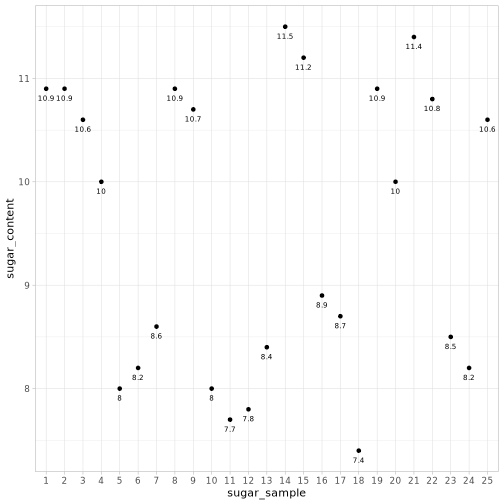
\includegraphics{note_stat501_files/figure-latex/unnamed-chunk-1-1.pdf}

\begin{Shaded}
\begin{Highlighting}[]

\NormalTok{finney <-}\StringTok{ }\KeywordTok{data.frame}\NormalTok{(Finney[}\DecValTok{1}\OperatorTok{:}\DecValTok{3}\NormalTok{])}
\NormalTok{finney[,}\DecValTok{3}\NormalTok{] <-}\StringTok{ }\KeywordTok{as.factor}\NormalTok{(finney[,}\DecValTok{3}\NormalTok{])}
\KeywordTok{table}\NormalTok{(finney[}\DecValTok{3}\NormalTok{])}
\CommentTok{## }
\CommentTok{##  0  1 }
\CommentTok{## 19 20}
\NormalTok{n <-}\StringTok{ }\KeywordTok{nrow}\NormalTok{(finney)}
\end{Highlighting}
\end{Shaded}

The starting value \(\beta^{(0)}\) is the least square estimate
\((\mathbf{X}^T\mathbf{X})^{-1}\mathbf{X}^T\mathbf{y}\)

\begin{Shaded}
\begin{Highlighting}[]
\CommentTok{# X <- cbind(Vol, Rate)}
\CommentTok{# (beta <- solve( t(X) %*% X ) %*% t(X) %*% Resp) #start from LS estimate}
\NormalTok{X <-}\StringTok{ }\KeywordTok{cbind}\NormalTok{(}\DecValTok{1}\NormalTok{, Vol, Rate)}
\NormalTok{(beta <-}\StringTok{ }\KeywordTok{as.vector}\NormalTok{(}\KeywordTok{solve}\NormalTok{( }\KeywordTok{t}\NormalTok{(X) }\OperatorTok\StringTok{ }\NormalTok{X ) }\OperatorTok\StringTok{ }\KeywordTok{t}\NormalTok{(X) }\OperatorTok\StringTok{ }\NormalTok{Resp))}
\CommentTok{## [1] -0.6097  0.3974  0.3433}
\NormalTok{p <-}\StringTok{ }\KeywordTok{dim}\NormalTok{(X)[}\DecValTok{2}\NormalTok{]}
\end{Highlighting}
\end{Shaded}

\(\mu=\mathbf{x}_i^T\boldsymbol{\beta}\)

\begin{Shaded}
\begin{Highlighting}[]
\NormalTok{(mu <-}\StringTok{ }\KeywordTok{as.vector}\NormalTok{(X }\OperatorTok\StringTok{ }\NormalTok{beta)) }\CommentTok{# Initial mu of Z}
\CommentTok{##  [1]  1.143927  1.155416  0.745264  0.203263  0.806730  0.869976 -0.113819  0.411018  0.005407 -0.097580 -0.096127  0.552894  0.658588  0.746518  0.975669  0.867323  1.211269  0.213825  0.429763  0.723541  0.235812  0.234686  0.390221  0.453267  0.637191  0.143650  0.620553  0.420064  0.471485  0.163448  0.720761  0.427183  0.455646  0.582664  0.553748  0.851358  0.420064  0.340580  0.464755}
\end{Highlighting}
\end{Shaded}

\(Z_i|\boldsymbol{y,\beta}\sim N(\mathbf{x}_i^T\boldsymbol{\beta},1)\)
truncated by 0 at the
\(\begin{cases}\text{left if}&y_i=1\\\text{right if}&y_i=0\end{cases}\)

\begin{Shaded}
\begin{Highlighting}[]
\CommentTok{# only works for the second probit model}
\NormalTok{ez<-}\KeywordTok{as.vector}\NormalTok{(X}\OperatorTok\NormalTok{beta)}
\KeywordTok{set.seed}\NormalTok{(}\DecValTok{123}\NormalTok{); u<-}\KeywordTok{runif}\NormalTok{(n,}\DecValTok{0}\NormalTok{,}\DecValTok{1}\NormalTok{)}
\NormalTok{(z<-}\StringTok{ }\NormalTok{ez }\OperatorTok{+}\StringTok{ }\KeywordTok{qnorm}\NormalTok{(}\KeywordTok{ifelse}\NormalTok{(Resp}\OperatorTok{==}\DecValTok{1}\NormalTok{,u}\OperatorTok{+}\NormalTok{(}\DecValTok{1}\OperatorTok{-}\NormalTok{u)}\OperatorTok{*}\KeywordTok{pnorm}\NormalTok{(}\DecValTok{0}\NormalTok{,ez,}\DecValTok{1}\NormalTok{),u}\OperatorTok{*}\KeywordTok{pnorm}\NormalTok{(}\DecValTok{0}\NormalTok{,ez,}\DecValTok{1}\NormalTok{))))}
\CommentTok{##  [1]  0.832073  2.050193  0.855184  1.694783  2.481027  0.127697 -0.673112 -0.102212 -0.593768 -0.784538 -0.058383 -0.566233 -0.284434  1.186252  0.303054  2.266680  0.774671  0.062684 -0.799845  2.537792 -0.117693 -0.341846 -0.371826 -0.005182  1.298868 -0.341458  1.049459 -0.420286  0.510766 -1.358535  2.627659 -0.091675 -0.303070  1.630959  0.050385  1.055347 -0.236386 -1.068817  0.557838}
\end{Highlighting}
\end{Shaded}

\begin{Shaded}
\begin{Highlighting}[]
\CommentTok{# only works for the first probit model}
\NormalTok{tr_norm<-}\ControlFlowTok{function}\NormalTok{(n,mu,v,}\DataTypeTok{truc_side=}\StringTok{'left'}\NormalTok{)\{ }\CommentTok{# Truncated Normal function}
\NormalTok{u<-}\KeywordTok{runif}\NormalTok{(n,}\DataTypeTok{min=}\DecValTok{0}\NormalTok{,}\DataTypeTok{max=}\DecValTok{1}\NormalTok{)}
  \ControlFlowTok{if}\NormalTok{(truc_side}\OperatorTok{==}\StringTok{'left'}\NormalTok{)\{}
\NormalTok{ tr_norm_value<-u}\OperatorTok{-}\NormalTok{u}\OperatorTok{*}\KeywordTok{pnorm}\NormalTok{(}\DecValTok{0}\NormalTok{,}\DataTypeTok{mean=}\NormalTok{mu,}\DataTypeTok{sd=}\KeywordTok{sqrt}\NormalTok{(v))}\OperatorTok{+}\KeywordTok{pnorm}\NormalTok{(}\DecValTok{0}\NormalTok{,}\DataTypeTok{mean=}\NormalTok{mu,}\DataTypeTok{sd=}\KeywordTok{sqrt}\NormalTok{(v))\}}
 \ControlFlowTok{if}\NormalTok{(truc_side}\OperatorTok{==}\StringTok{'right'}\NormalTok{)\{}
\NormalTok{   tr_norm_value<-u}\OperatorTok{*}\KeywordTok{pnorm}\NormalTok{(}\DecValTok{0}\NormalTok{,}\DataTypeTok{mean=}\NormalTok{mu,}\DataTypeTok{sd=}\KeywordTok{sqrt}\NormalTok{(v))\}}
  \KeywordTok{qnorm}\NormalTok{(tr_norm_value,mu,}\KeywordTok{sqrt}\NormalTok{(v))}
\NormalTok{\}}

\KeywordTok{set.seed}\NormalTok{(}\DecValTok{123}\NormalTok{)}
\NormalTok{(z<-}\StringTok{ }\KeywordTok{ifelse}\NormalTok{(Resp}\OperatorTok{==}\DecValTok{1}\NormalTok{, }\CommentTok{# Initial Z}
\KeywordTok{tr_norm}\NormalTok{(}\DecValTok{1}\NormalTok{,mu,}\DecValTok{1}\NormalTok{),}
\KeywordTok{tr_norm}\NormalTok{(}\DecValTok{1}\NormalTok{,mu,}\DecValTok{1}\NormalTok{,}\StringTok{'right'}\NormalTok{)}
\NormalTok{))}
\CommentTok{##  [1]  0.8321  0.8391  0.6197  0.4216  0.6485  0.6795 -0.2905 -0.2065 -0.2675 -0.2872 -0.2869 -0.1901 -0.1792  0.6203  0.7349  0.6782  0.8741  0.4246 -0.2042  0.6099 -0.2300 -0.2302 -0.2091 -0.2014  0.5726 -0.2440  0.5657 -0.2054  0.5081 -0.2409  0.6087 -0.2045 -0.2011  0.5503  0.5389  0.6702 -0.2054 -0.2155  0.5056}
\end{Highlighting}
\end{Shaded}

\emph{other attempts of sampling from truncated normal}

\begin{Shaded}
\begin{Highlighting}[]

\CommentTok{#for(j in 1:n)\{  }
\CommentTok{#ifelse(Resp[j]==1,}
\CommentTok{#z[j] <- rtruncnorm(1,a=0,b=Inf,mean=mu[j],sd=1),}
\CommentTok{#z[j] <- rtruncnorm(1,a=Inf,b=0,mean=mu[j],sd=1)}
\CommentTok{#)}
\CommentTok{#\}}

\CommentTok{# anohter attempt of truncated}
\CommentTok{#z<- abs(rnorm(n,mean=mu,sd=1)),}
\CommentTok{#z<- -abs(rnorm(n,mean=mu,sd=1))}
\end{Highlighting}
\end{Shaded}

\(\boldsymbol{\hat\beta_Z}=(\mathbf{X}^T\mathbf{X})^{-1}\mathbf{X}^T\mathbf{Z}\)

\(\Omega=(\mathbf{X}^T\mathbf{X})^{-1})\)

\begin{Shaded}
\begin{Highlighting}[]
\KeywordTok{solve}\NormalTok{(}\KeywordTok{t}\NormalTok{(X)}\OperatorTok\NormalTok{X)}\OperatorTok\KeywordTok{t}\NormalTok{(X)}\OperatorTok\NormalTok{z }\CommentTok{# first mu for Beta}
\CommentTok{##         [,1]}
\CommentTok{##      -0.9472}
\CommentTok{## Vol   0.4217}
\CommentTok{## Rate  0.3444}
\KeywordTok{solve}\NormalTok{(}\KeywordTok{t}\NormalTok{(X)}\OperatorTok\NormalTok{X)            }\CommentTok{# first omega for Beta}
\CommentTok{##                    Vol     Rate}
\CommentTok{##       0.32203 -0.09689 -0.09709}
\CommentTok{## Vol  -0.09689  0.04789  0.01873}
\CommentTok{## Rate -0.09709  0.01873  0.04224}

\NormalTok{iXX<-}\KeywordTok{solve}\NormalTok{(}\KeywordTok{t}\NormalTok{(X)}\OperatorTok\NormalTok{X)  ; V<-iXX}\OperatorTok{*}\NormalTok{(n}\OperatorTok{/}\NormalTok{(n}\OperatorTok{+}\DecValTok{1}\NormalTok{)) ; cholV<-}\KeywordTok{chol}\NormalTok{(V) }\CommentTok{# from Hoff (2009, Ch.12)}
\end{Highlighting}
\end{Shaded}

\hypertarget{the-first-gibbs-sampling}{%
\paragraph{The first Gibbs sampling}\label{the-first-gibbs-sampling}}

\begin{Shaded}
\begin{Highlighting}[]
\NormalTok{M <-}\StringTok{ }\DecValTok{2500}\NormalTok{; }\KeywordTok{set.seed}\NormalTok{(}\DecValTok{123}\NormalTok{)}
\NormalTok{Gibbs <-}\StringTok{ }\KeywordTok{matrix}\NormalTok{(}\OtherTok{NA}\NormalTok{,}\DataTypeTok{ncol=}\NormalTok{p,}\DataTypeTok{nrow=}\NormalTok{M); ZZ<-}\KeywordTok{matrix}\NormalTok{(}\OtherTok{NA}\NormalTok{,M,n)      }\CommentTok{#For full Sample}
\NormalTok{gibbs <-}\StringTok{ }\KeywordTok{matrix}\NormalTok{(}\OtherTok{NA}\NormalTok{,}\DataTypeTok{ncol=}\NormalTok{p,}\DataTypeTok{nrow=}\DecValTok{100}\NormalTok{); Z<-}\KeywordTok{matrix}\NormalTok{(}\OtherTok{NA}\NormalTok{,}\DecValTok{100}\NormalTok{,n) }\CommentTok{#For Sub Sample}
\ControlFlowTok{for}\NormalTok{(m }\ControlFlowTok{in} \DecValTok{1}\OperatorTok{:}\NormalTok{M)\{  }\CommentTok{#Gibbs Sampler}
  
\CommentTok{# beta <- mvrnorm(1, solve(t(X)%*%X)%*%(t(X)%*%z), solve(t(X)%*%X)) # without n/(n+1)}
\NormalTok{beta <-}\StringTok{ }\KeywordTok{mvrnorm}\NormalTok{(}\DecValTok{1}\NormalTok{, V}\OperatorTok\NormalTok{(}\KeywordTok{t}\NormalTok{(X)}\OperatorTok\NormalTok{z), V) }\CommentTok{# draw beta from Normal}

\NormalTok{z<-}\StringTok{ }\KeywordTok{ifelse}\NormalTok{(Resp}\OperatorTok{==}\DecValTok{1}\NormalTok{, }\CommentTok{# draw Z from truncated Normal}
\KeywordTok{tr_norm}\NormalTok{(}\DecValTok{1}\NormalTok{ ,}\KeywordTok{t}\NormalTok{(X }\OperatorTok\StringTok{ }\NormalTok{beta), }\DecValTok{1}\NormalTok{),}
\KeywordTok{tr_norm}\NormalTok{(}\DecValTok{1}\NormalTok{ ,}\KeywordTok{t}\NormalTok{(X }\OperatorTok\StringTok{ }\NormalTok{beta), }\DecValTok{1}\NormalTok{ ,}\StringTok{'right'}\NormalTok{)}
\NormalTok{)}

\CommentTok{#ez<-(X%*%beta)}
\CommentTok{#u<-runif(n,0,1)}
\CommentTok{#z<- ez + qnorm(ifelse(Resp==1,u+(1-u)*pnorm(0,ez,1),u*pnorm(0,ez,1)))}

\NormalTok{Gibbs[m,] <-}\StringTok{ }\KeywordTok{t}\NormalTok{(beta); ZZ[m,]<-}\StringTok{ }\NormalTok{z                                        }\CommentTok{# full samples}
\ControlFlowTok{if}\NormalTok{(m}\OperatorTok\NormalTok{(M}\OperatorTok{/}\DecValTok{100}\NormalTok{)}\OperatorTok{==}\DecValTok{0}\NormalTok{) \{ gibbs[m}\OperatorTok{/}\NormalTok{(M}\OperatorTok{/}\DecValTok{100}\NormalTok{),] <-}\StringTok{ }\KeywordTok{t}\NormalTok{(beta); Z[m}\OperatorTok{/}\NormalTok{(M}\OperatorTok{/}\DecValTok{100}\NormalTok{),]<-}\StringTok{ }\NormalTok{z\}   }\CommentTok{# subsamples of equal size}
\NormalTok{\}}
\end{Highlighting}
\end{Shaded}

\(\boldsymbol{\hat\beta}\approx\frac1m\sum_{i=1}^m(\boldsymbol{\beta|Z^{(i)}})\)

\begin{Shaded}
\begin{Highlighting}[]
\NormalTok{full.mean <-}\StringTok{ }\KeywordTok{colMeans}\NormalTok{(Gibbs[,])}
\NormalTok{burnin <-}\StringTok{ }\DecValTok{2400}\OperatorTok{:}\DecValTok{2500}
\NormalTok{tail.mean <-}\StringTok{ }\KeywordTok{colMeans}\NormalTok{(Gibbs[burnin,])}
\NormalTok{sub.mean <-}\StringTok{ }\KeywordTok{colMeans}\NormalTok{(gibbs)}
\NormalTok{par<-}\StringTok{ }\KeywordTok{cbind}\NormalTok{(full.mean,tail.mean,sub.mean)}
\KeywordTok{rownames}\NormalTok{(par) <-}\StringTok{ }\KeywordTok{c}\NormalTok{(}\StringTok{"Beta0"}\NormalTok{,}\StringTok{"Beta1"}\NormalTok{,}\StringTok{"Beta2"}\NormalTok{)}
\NormalTok{pander}\OperatorTok{::}\KeywordTok{pander}\NormalTok{(}\KeywordTok{round}\NormalTok{((par),}\DecValTok{4}\NormalTok{))}
\end{Highlighting}
\end{Shaded}

\begin{longtable}[]{@{}cccc@{}}
\toprule
\begin{minipage}[b]{0.15\columnwidth}\centering
~\strut
\end{minipage} & \begin{minipage}[b]{0.15\columnwidth}\centering
full.mean\strut
\end{minipage} & \begin{minipage}[b]{0.15\columnwidth}\centering
tail.mean\strut
\end{minipage} & \begin{minipage}[b]{0.15\columnwidth}\centering
sub.mean\strut
\end{minipage}\tabularnewline
\midrule
\endhead
\begin{minipage}[t]{0.15\columnwidth}\centering
\textbf{Beta0}\strut
\end{minipage} & \begin{minipage}[t]{0.15\columnwidth}\centering
-5.417\strut
\end{minipage} & \begin{minipage}[t]{0.15\columnwidth}\centering
-6.043\strut
\end{minipage} & \begin{minipage}[t]{0.15\columnwidth}\centering
-5.371\strut
\end{minipage}\tabularnewline
\begin{minipage}[t]{0.15\columnwidth}\centering
\textbf{Beta1}\strut
\end{minipage} & \begin{minipage}[t]{0.15\columnwidth}\centering
2.133\strut
\end{minipage} & \begin{minipage}[t]{0.15\columnwidth}\centering
2.45\strut
\end{minipage} & \begin{minipage}[t]{0.15\columnwidth}\centering
2.112\strut
\end{minipage}\tabularnewline
\begin{minipage}[t]{0.15\columnwidth}\centering
\textbf{Beta2}\strut
\end{minipage} & \begin{minipage}[t]{0.15\columnwidth}\centering
1.586\strut
\end{minipage} & \begin{minipage}[t]{0.15\columnwidth}\centering
1.766\strut
\end{minipage} & \begin{minipage}[t]{0.15\columnwidth}\centering
1.566\strut
\end{minipage}\tabularnewline
\bottomrule
\end{longtable}

\begin{Shaded}
\begin{Highlighting}[]
\NormalTok{full.quant <-}\StringTok{ }\KeywordTok{apply}\NormalTok{(Gibbs[burnin,],}\DecValTok{2}\NormalTok{,quantile,}\DataTypeTok{probs=}\KeywordTok{c}\NormalTok{(}\FloatTok{0.025}\NormalTok{,}\FloatTok{0.5}\NormalTok{,}\FloatTok{0.975}\NormalTok{)) }
\NormalTok{tail.quant <-}\StringTok{ }\KeywordTok{apply}\NormalTok{(Gibbs[burnin,],}\DecValTok{2}\NormalTok{,quantile,}\DataTypeTok{probs=}\KeywordTok{c}\NormalTok{(}\FloatTok{0.025}\NormalTok{,}\FloatTok{0.5}\NormalTok{,}\FloatTok{0.975}\NormalTok{)) }
\NormalTok{sub.quant <-}\StringTok{ }\KeywordTok{apply}\NormalTok{(gibbs,}\DecValTok{2}\NormalTok{,quantile,}\DataTypeTok{probs=}\KeywordTok{c}\NormalTok{(}\FloatTok{0.025}\NormalTok{,}\FloatTok{0.5}\NormalTok{,}\FloatTok{0.975}\NormalTok{)) }
\NormalTok{par<-}\StringTok{ }\KeywordTok{rbind}\NormalTok{(full.quant,tail.quant,sub.quant)}
\KeywordTok{colnames}\NormalTok{(par) <-}\StringTok{ }\KeywordTok{c}\NormalTok{(}\StringTok{"Beta0"}\NormalTok{,}\StringTok{"Beta1"}\NormalTok{,}\StringTok{"Beta2"}\NormalTok{)}
\NormalTok{pander}\OperatorTok{::}\KeywordTok{pander}\NormalTok{(}\KeywordTok{round}\NormalTok{(}\KeywordTok{t}\NormalTok{(par),}\DecValTok{4}\NormalTok{))}
\end{Highlighting}
\end{Shaded}

\begin{Shaded}
\begin{Highlighting}[]
\KeywordTok{par}\NormalTok{(}\DataTypeTok{mar=}\KeywordTok{c}\NormalTok{(}\DecValTok{5}\NormalTok{,}\DecValTok{3}\NormalTok{,}\DecValTok{1}\NormalTok{,}\DecValTok{1}\NormalTok{),}\DataTypeTok{mgp=}\KeywordTok{c}\NormalTok{(}\FloatTok{1.75}\NormalTok{,.}\DecValTok{75}\NormalTok{,}\DecValTok{0}\NormalTok{)); }\KeywordTok{par}\NormalTok{(}\DataTypeTok{mfrow=}\KeywordTok{c}\NormalTok{(}\DecValTok{3}\NormalTok{,}\DecValTok{3}\NormalTok{))}
\NormalTok{lab<-}\KeywordTok{c}\NormalTok{(}\KeywordTok{expression}\NormalTok{(beta[}\DecValTok{0}\NormalTok{]),}\KeywordTok{expression}\NormalTok{(beta[}\DecValTok{1}\NormalTok{]),}\KeywordTok{expression}\NormalTok{(beta[}\DecValTok{2}\NormalTok{]))}
\ControlFlowTok{for}\NormalTok{(j }\ControlFlowTok{in} \DecValTok{1}\OperatorTok{:}\DecValTok{3}\NormalTok{) \{}
\KeywordTok{acf}\NormalTok{(Gibbs[,j],}\DataTypeTok{ci.col=}\StringTok{"dodgerblue4"}\NormalTok{,}\DataTypeTok{xlab=}\NormalTok{lab[j])\}  }
\ControlFlowTok{for}\NormalTok{(j }\ControlFlowTok{in} \DecValTok{1}\OperatorTok{:}\DecValTok{3}\NormalTok{) \{}
\KeywordTok{acf}\NormalTok{(Gibbs[burnin,j],}\DataTypeTok{ci.col=}\StringTok{"dodgerblue4"}\NormalTok{,}\DataTypeTok{xlab=}\NormalTok{lab[j])\} }
\ControlFlowTok{for}\NormalTok{(j }\ControlFlowTok{in} \DecValTok{1}\OperatorTok{:}\DecValTok{3}\NormalTok{) \{}
\KeywordTok{acf}\NormalTok{(gibbs[,j],}\DataTypeTok{xlab=}\NormalTok{lab[j],}\DataTypeTok{ci.col=}\StringTok{"dodgerblue4"}\NormalTok{)\}}
\KeywordTok{mtext}\NormalTok{(}\StringTok{"autocorrelation functions with Gibbs1.full(above),Gibbs1.tail(middle) ,Gibbs1.sub(below)"}\NormalTok{,}\DataTypeTok{side=}\DecValTok{1}\NormalTok{,}\DataTypeTok{line=}\OperatorTok{-}\DecValTok{1}\NormalTok{,}\DataTypeTok{outer=}\NormalTok{T)}
\end{Highlighting}
\end{Shaded}

\begin{center}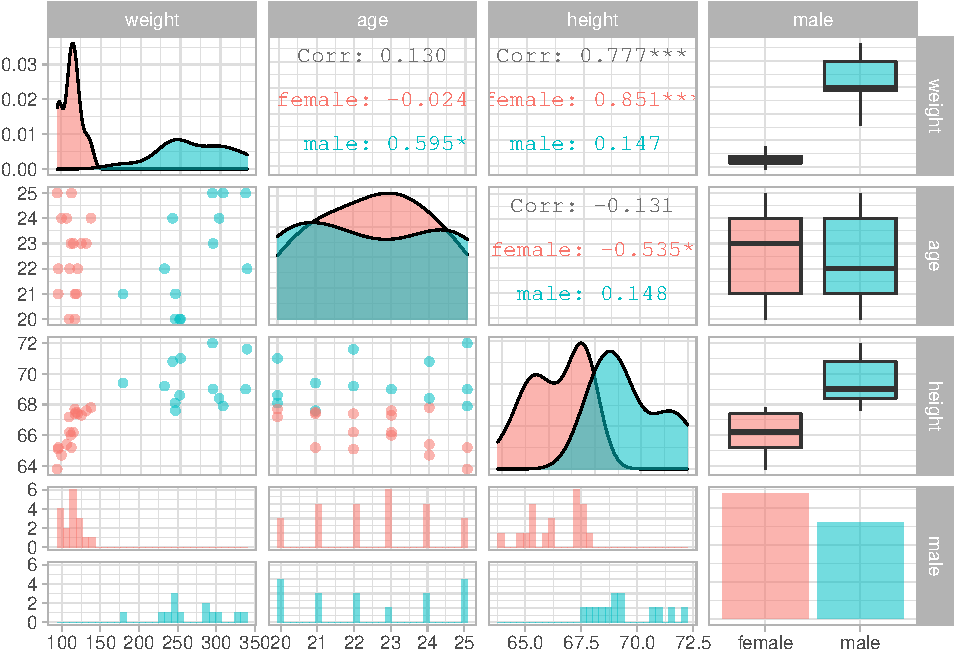
\includegraphics{note_stat501_files/figure-latex/unnamed-chunk-11-1} \end{center}

Choose sub-sampling

\begin{Shaded}
\begin{Highlighting}[]
\KeywordTok{par}\NormalTok{(}\DataTypeTok{mfrow=}\KeywordTok{c}\NormalTok{(}\DecValTok{3}\NormalTok{,}\DecValTok{3}\NormalTok{),}\DataTypeTok{mar=}\KeywordTok{c}\NormalTok{(}\DecValTok{3}\NormalTok{,}\FloatTok{3.2}\NormalTok{,.}\DecValTok{5}\NormalTok{,.}\DecValTok{5}\NormalTok{),}\DataTypeTok{mgp=}\KeywordTok{c}\NormalTok{(}\FloatTok{1.70}\NormalTok{,.}\DecValTok{70}\NormalTok{,}\DecValTok{0}\NormalTok{))}
\ControlFlowTok{for}\NormalTok{(j }\ControlFlowTok{in} \DecValTok{1}\OperatorTok{:}\NormalTok{p)\{}
\KeywordTok{plot}\NormalTok{(gibbs[,j],  }\DataTypeTok{ylab=}\NormalTok{lab[j],}\DataTypeTok{main=}\StringTok{""}\NormalTok{,}\DataTypeTok{pch=}\DecValTok{1}\NormalTok{,}\DataTypeTok{cex=}\FloatTok{0.1}\NormalTok{,}
     \DataTypeTok{xlab=}\StringTok{"Gibbs iteration (k)"}\NormalTok{,}\DataTypeTok{col=}\StringTok{"cornflowerblue"}\NormalTok{)  }
\KeywordTok{plot}\NormalTok{(}\KeywordTok{cumsum}\NormalTok{(gibbs[,j])}\OperatorTok{/}\NormalTok{(}\DecValTok{1}\OperatorTok{:}\DecValTok{100}\NormalTok{),  }\DataTypeTok{ylab=}\NormalTok{lab[j],}\DataTypeTok{main=}\StringTok{""}\NormalTok{,}
     \DataTypeTok{type=}\StringTok{"l"}\NormalTok{,}\DataTypeTok{col=}\StringTok{"cornflowerblue"}\NormalTok{,}\DataTypeTok{lwd=}\DecValTok{2}\NormalTok{,}\DataTypeTok{pch=}\DecValTok{20}\NormalTok{,}\DataTypeTok{cex=}\FloatTok{0.7}\NormalTok{,}\DataTypeTok{xlab=}\StringTok{"Gibbs iteration (k)"}\NormalTok{)}
\CommentTok{#hist(gibbs.mat[-burnin,j],freq =F,xlab=paste("distribution of est. for beta",j-1),}
\CommentTok{#     main="",col="cornflowerblue")}
\KeywordTok{plot}\NormalTok{(}\KeywordTok{density}\NormalTok{(gibbs[,j],}\DataTypeTok{adj=}\DecValTok{2}\NormalTok{),}\DataTypeTok{lwd=}\DecValTok{2}\NormalTok{,}\DataTypeTok{main=}\StringTok{""}\NormalTok{,}\DataTypeTok{col=}\StringTok{"cornflowerblue"}\NormalTok{,}
    \DataTypeTok{xlab=}\NormalTok{lab[j],}\DataTypeTok{ylab=}\StringTok{"density"}\NormalTok{)}
\KeywordTok{abline}\NormalTok{(}\DataTypeTok{v=}\KeywordTok{quantile}\NormalTok{(gibbs[,j],}\KeywordTok{c}\NormalTok{(}\FloatTok{0.025}\NormalTok{,}\FloatTok{0.975}\NormalTok{)),}\DataTypeTok{col=}\StringTok{"gray"}\NormalTok{,}\DataTypeTok{lwd=}\DecValTok{1}\NormalTok{)}
\NormalTok{\}}
\end{Highlighting}
\end{Shaded}

\begin{center}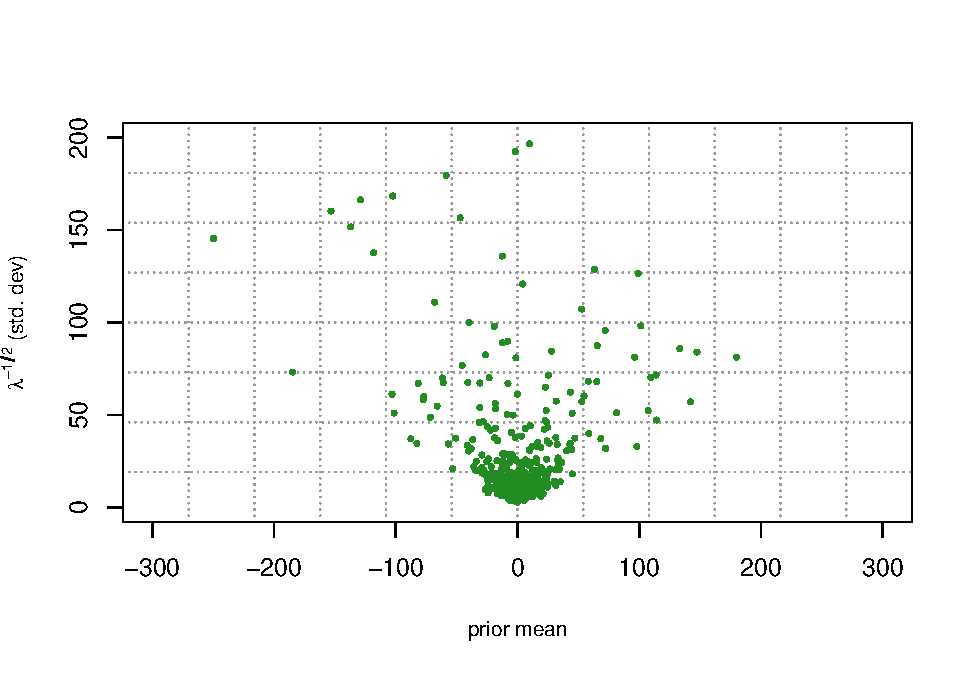
\includegraphics{note_stat501_files/figure-latex/unnamed-chunk-12-1} \end{center}

\(p_i=\Phi(\mathbf{x}_i^T\boldsymbol{\beta})\)

\begin{Shaded}
\begin{Highlighting}[]
\NormalTok{(prob <-}\StringTok{ }\KeywordTok{pnorm}\NormalTok{(}\KeywordTok{t}\NormalTok{(X }\OperatorTok\StringTok{ }\NormalTok{beta),}\DecValTok{0}\NormalTok{,}\DecValTok{1}\NormalTok{))}
\CommentTok{##      [,1] [,2]   [,3]     [,4] [,5]   [,6]         [,7]   [,8]       [,9]        [,10]        [,11]  [,12]  [,13]  [,14]  [,15]  [,16] [,17]    [,18] [,19]  [,20]    [,21]   [,22] [,23]  [,24]  [,25]     [,26]  [,27]  [,28]  [,29]    [,30]  [,31]  [,32] [,33]  [,34]  [,35]  [,36]  [,37]   [,38]  [,39]}
\CommentTok{## [1,]    1    1 0.9645 0.004525 0.98 0.9936 0.0000001507 0.2008 0.00002489 0.0000006221 0.0000005118 0.4913 0.7927 0.9706 0.9996 0.9995     1 0.006583 0.346 0.9721 0.005637 0.01163 0.191 0.3764 0.8747 0.0008358 0.8687 0.1994 0.5096 0.006326 0.9903 0.4631  0.31 0.6847 0.6211 0.9917 0.1994 0.06003 0.3721}
\end{Highlighting}
\end{Shaded}

\hypertarget{the-second-gibbs-sampling-refer-to-hoff-2009-ch.12}{%
\paragraph{The second Gibbs sampling, refer to (Hoff, 2009,
Ch.12)}\label{the-second-gibbs-sampling-refer-to-hoff-2009-ch.12}}

\begin{Shaded}
\begin{Highlighting}[]
\NormalTok{iXX<-}\KeywordTok{solve}\NormalTok{(}\KeywordTok{t}\NormalTok{(X)}\OperatorTok\NormalTok{X)  ; V<-iXX}\OperatorTok{*}\NormalTok{(n}\OperatorTok{/}\NormalTok{(n}\OperatorTok{+}\DecValTok{1}\NormalTok{)) ; cholV<-}\KeywordTok{chol}\NormalTok{(V)}
\end{Highlighting}
\end{Shaded}

\begin{Shaded}
\begin{Highlighting}[]
\CommentTok{#### probit regression}
\CommentTok{## setup}
\KeywordTok{set.seed}\NormalTok{(}\DecValTok{123}\NormalTok{)}
\NormalTok{beta<-}\KeywordTok{rep}\NormalTok{(}\DecValTok{0}\NormalTok{,p) }
\NormalTok{z<-}\KeywordTok{qnorm}\NormalTok{(}\KeywordTok{rank}\NormalTok{(Resp,}\DataTypeTok{ties.method=}\StringTok{"random"}\NormalTok{)}\OperatorTok{/}\NormalTok{(n}\OperatorTok{+}\DecValTok{1}\NormalTok{)) }\CommentTok{# random initial Z}
\NormalTok{BETA<-}\KeywordTok{matrix}\NormalTok{(}\OtherTok{NA}\NormalTok{,}\DecValTok{100}\NormalTok{,p) ; Z<-}\KeywordTok{matrix}\NormalTok{(}\OtherTok{NA}\NormalTok{,}\DecValTok{100}\NormalTok{,n) ; ac<-}\DecValTok{0}
\NormalTok{mu<-}\DecValTok{0}\NormalTok{ ; sigma<-}\DecValTok{100}  \CommentTok{### Why????}

\CommentTok{## MCMC}
\NormalTok{S<-}\DecValTok{2500}
\ControlFlowTok{for}\NormalTok{(s }\ControlFlowTok{in} \DecValTok{1}\OperatorTok{:}\NormalTok{S) }
\NormalTok{\{}
  \CommentTok{#update beta}
\NormalTok{  E<-}\StringTok{ }\NormalTok{V}\OperatorTok\NormalTok{( }\KeywordTok{t}\NormalTok{(X)}\OperatorTok\NormalTok{z )}
\NormalTok{  beta<-}\StringTok{ }\NormalTok{cholV}\OperatorTok\KeywordTok{rnorm}\NormalTok{(p) }\OperatorTok{+}\StringTok{ }\NormalTok{E  }\CommentTok{# ????????}

  \CommentTok{#update z}
\NormalTok{  ez<-X}\OperatorTok\NormalTok{beta}
\NormalTok{  u<-}\KeywordTok{runif}\NormalTok{(n,}\DecValTok{0}\NormalTok{,}\DecValTok{1}\NormalTok{)}
\NormalTok{  z<-}\StringTok{ }\NormalTok{ez }\OperatorTok{+}\StringTok{ }\KeywordTok{qnorm}\NormalTok{(}\KeywordTok{ifelse}\NormalTok{(Resp}\OperatorTok{==}\DecValTok{1}\NormalTok{,u}\OperatorTok{+}\NormalTok{(}\DecValTok{1}\OperatorTok{-}\NormalTok{u)}\OperatorTok{*}\KeywordTok{pnorm}\NormalTok{(}\DecValTok{0}\NormalTok{,ez,}\DecValTok{1}\NormalTok{),u}\OperatorTok{*}\KeywordTok{pnorm}\NormalTok{(}\DecValTok{0}\NormalTok{,ez,}\DecValTok{1}\NormalTok{)))}
    
  \CommentTok{#help mixing}
\NormalTok{c<-}\KeywordTok{rnorm}\NormalTok{(}\DecValTok{1}\NormalTok{,}\DecValTok{0}\NormalTok{,n}\OperatorTok{^}\NormalTok{(}\OperatorTok{-}\DecValTok{1}\OperatorTok{/}\DecValTok{3}\NormalTok{))  }\CommentTok{#  sd responding the sample size ????}
\NormalTok{zp<-z}\OperatorTok{+}\NormalTok{c }\CommentTok{#;g <- 0 ; gp<-g+c}
\NormalTok{lhr<-}\StringTok{  }\KeywordTok{sum}\NormalTok{(}\KeywordTok{dnorm}\NormalTok{(zp,ez,}\DecValTok{1}\NormalTok{,}\DataTypeTok{log=}\NormalTok{T) }\OperatorTok{-}\StringTok{ }\KeywordTok{dnorm}\NormalTok{(z,ez,}\DecValTok{1}\NormalTok{,}\DataTypeTok{log=}\NormalTok{T) ) }\CommentTok{#+ sum(dnorm(c,mu,sigma,log=T) - dnorm(0,mu,sigma,log=T) )}
\ControlFlowTok{if}\NormalTok{(}\KeywordTok{log}\NormalTok{(}\KeywordTok{runif}\NormalTok{(}\DecValTok{1}\NormalTok{))}\OperatorTok{<}\NormalTok{lhr) \{ z<-zp ; ac<-ac}\OperatorTok{+}\DecValTok{1}\NormalTok{ \}              }\CommentTok{# ; g<-gp}

  \ControlFlowTok{if}\NormalTok{(s}\OperatorTok\NormalTok{(S}\OperatorTok{/}\DecValTok{100}\NormalTok{)}\OperatorTok{==}\DecValTok{0}\NormalTok{) }
\NormalTok{  \{ }
    \CommentTok{# cat(s/S,ac/s,"\textbackslash{}n")}
\NormalTok{    BETA[s}\OperatorTok{/}\NormalTok{(S}\OperatorTok{/}\DecValTok{100}\NormalTok{),]<-}\StringTok{  }\NormalTok{beta}
\NormalTok{    Z[s}\OperatorTok{/}\NormalTok{(S}\OperatorTok{/}\DecValTok{100}\NormalTok{),]<-}\StringTok{ }\NormalTok{z}
\NormalTok{  \}}
\NormalTok{\} }
\end{Highlighting}
\end{Shaded}

\begin{Shaded}
\begin{Highlighting}[]
\NormalTok{(beta.pm<-}\KeywordTok{apply}\NormalTok{(BETA,}\DecValTok{2}\NormalTok{,mean))}
\end{Highlighting}
\end{Shaded}

\begin{verbatim}
## [1] -5.124  2.006  1.503
\end{verbatim}

\begin{Shaded}
\begin{Highlighting}[]
\KeywordTok{par}\NormalTok{(}\DataTypeTok{mfrow=}\KeywordTok{c}\NormalTok{(}\DecValTok{1}\NormalTok{,}\DecValTok{3}\NormalTok{),}\DataTypeTok{mar=}\KeywordTok{c}\NormalTok{(}\DecValTok{3}\NormalTok{,}\FloatTok{3.2}\NormalTok{,.}\DecValTok{5}\NormalTok{,.}\DecValTok{5}\NormalTok{),}\DataTypeTok{mgp=}\KeywordTok{c}\NormalTok{(}\FloatTok{1.70}\NormalTok{,.}\DecValTok{70}\NormalTok{,}\DecValTok{0}\NormalTok{))}
\NormalTok{laby<-}\KeywordTok{c}\NormalTok{(}\StringTok{"density"}\NormalTok{,}\StringTok{""}\NormalTok{,}\StringTok{""}\NormalTok{)}
\ControlFlowTok{for}\NormalTok{(j }\ControlFlowTok{in} \DecValTok{1}\OperatorTok{:}\NormalTok{p)\{}
\KeywordTok{plot}\NormalTok{(}\KeywordTok{density}\NormalTok{(BETA[,j],}\DataTypeTok{adj=}\DecValTok{2}\NormalTok{),}\DataTypeTok{lwd=}\DecValTok{2}\NormalTok{,}\DataTypeTok{main=}\StringTok{""}\NormalTok{,}\CommentTok{#xlim=c(-10,5),}
    \DataTypeTok{xlab=}\NormalTok{lab[j],}\DataTypeTok{ylab=}\NormalTok{laby[j],}\DataTypeTok{col=}\StringTok{"cornflowerblue"}\NormalTok{)}
\NormalTok{sd<-}\KeywordTok{sqrt}\NormalTok{(  }\KeywordTok{solve}\NormalTok{(}\KeywordTok{t}\NormalTok{(X)}\OperatorTok\NormalTok{X}\OperatorTok{/}\NormalTok{n)[j,j] )}
\NormalTok{x<-}\KeywordTok{seq}\NormalTok{(}\KeywordTok{min}\NormalTok{(BETA[,j]),}\KeywordTok{max}\NormalTok{(BETA[,j]),}\DataTypeTok{length=}\DecValTok{100}\NormalTok{)}
\KeywordTok{lines}\NormalTok{(x,}\KeywordTok{dnorm}\NormalTok{(x,E[j],sd),}\DataTypeTok{lwd=}\DecValTok{2}\NormalTok{,}\DataTypeTok{col=}\StringTok{"gray"}\NormalTok{)}
\ControlFlowTok{if}\NormalTok{(j}\OperatorTok{==}\DecValTok{3}\NormalTok{) \{}\KeywordTok{legend}\NormalTok{(}\FloatTok{2.1}\NormalTok{,}\DecValTok{1}\NormalTok{,}\DataTypeTok{legend=}\KeywordTok{c}\NormalTok{(}\StringTok{"prior"}\NormalTok{,}\StringTok{"posterior"}\NormalTok{),}\DataTypeTok{lwd=}\KeywordTok{c}\NormalTok{(}\DecValTok{2}\NormalTok{,}\DecValTok{2}\NormalTok{),}\DataTypeTok{col=}\KeywordTok{c}\NormalTok{(}\StringTok{"gray"}\NormalTok{,}\StringTok{"cornflowerblue"}\NormalTok{),}\DataTypeTok{bty=}\StringTok{"n"}\NormalTok{)\}}
\NormalTok{\}}
\end{Highlighting}
\end{Shaded}

\begin{center}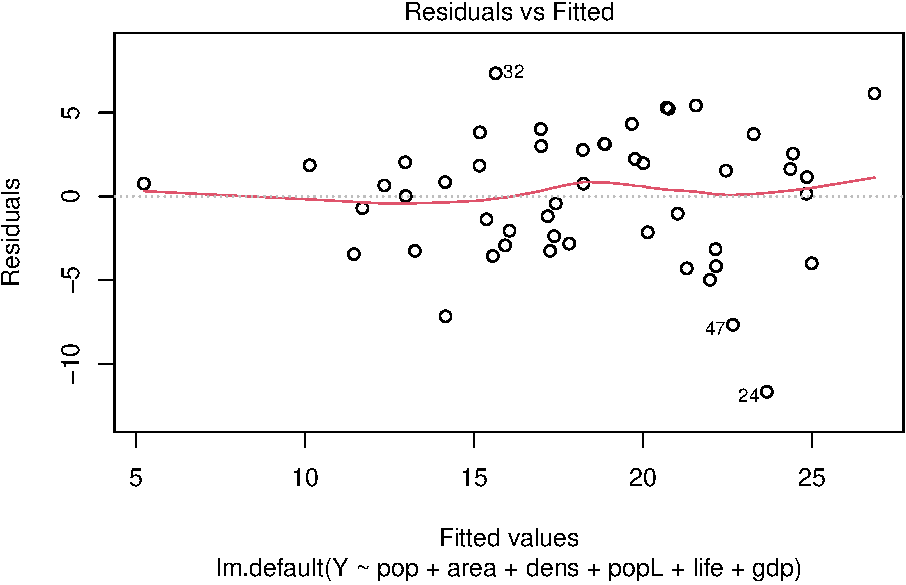
\includegraphics{note_stat501_files/figure-latex/unnamed-chunk-17-1} \end{center}

\begin{Shaded}
\begin{Highlighting}[]
\KeywordTok{source}\NormalTok{(}\StringTok{"rlreg.R"}\NormalTok{)}
\NormalTok{rfit<-}\KeywordTok{treg}\NormalTok{(Resp,X)}
\end{Highlighting}
\end{Shaded}

\begin{Shaded}
\begin{Highlighting}[]
\KeywordTok{par}\NormalTok{(}\DataTypeTok{mfrow=}\KeywordTok{c}\NormalTok{(}\DecValTok{1}\NormalTok{,}\DecValTok{3}\NormalTok{),}\DataTypeTok{mar=}\KeywordTok{c}\NormalTok{(}\DecValTok{3}\NormalTok{,}\FloatTok{3.2}\NormalTok{,.}\DecValTok{5}\NormalTok{,.}\DecValTok{5}\NormalTok{),}\DataTypeTok{mgp=}\KeywordTok{c}\NormalTok{(}\FloatTok{1.70}\NormalTok{,.}\DecValTok{70}\NormalTok{,}\DecValTok{0}\NormalTok{))}
\NormalTok{ymx<-}\KeywordTok{c}\NormalTok{(}\FloatTok{0.3}\NormalTok{,}\FloatTok{0.75}\NormalTok{,}\FloatTok{1.25}\NormalTok{)}
\ControlFlowTok{for}\NormalTok{(j }\ControlFlowTok{in} \DecValTok{1}\OperatorTok{:}\DecValTok{3}\NormalTok{) \{}
\KeywordTok{plot}\NormalTok{(}\KeywordTok{density}\NormalTok{(rfit}\OperatorTok{$}\NormalTok{BETA[,j],}\DataTypeTok{adj=}\DecValTok{2}\NormalTok{),}\DataTypeTok{lwd=}\DecValTok{2}\NormalTok{,}\DataTypeTok{main=}\StringTok{""}\NormalTok{,}
 \DataTypeTok{xlab=}\NormalTok{lab[j],}\DataTypeTok{col=}\StringTok{"gray"}\NormalTok{,}\DataTypeTok{ylim=}\KeywordTok{c}\NormalTok{(}\DecValTok{0}\NormalTok{,ymx[j]),}\DataTypeTok{ylab=}\NormalTok{laby[j])}
\KeywordTok{lines}\NormalTok{(}\KeywordTok{density}\NormalTok{(Gibbs[burnin,j],}\DataTypeTok{adj=}\DecValTok{2}\NormalTok{),}\DataTypeTok{col=}\StringTok{"cornflowerblue"}\NormalTok{,}\DataTypeTok{lwd=}\DecValTok{2}\NormalTok{)}
\KeywordTok{lines}\NormalTok{(}\KeywordTok{density}\NormalTok{(gibbs[,j],}\DataTypeTok{adj=}\DecValTok{2}\NormalTok{),}\DataTypeTok{col=}\StringTok{"cornflowerblue"}\NormalTok{,}\DataTypeTok{lwd=}\DecValTok{2}\NormalTok{,}\DataTypeTok{lty=}\DecValTok{2}\NormalTok{)}
\KeywordTok{lines}\NormalTok{(}\KeywordTok{density}\NormalTok{(BETA[,j],}\DataTypeTok{adj=}\DecValTok{2}\NormalTok{),}\DataTypeTok{col=}\StringTok{"cyan"}\NormalTok{,}\DataTypeTok{lwd=}\DecValTok{2}\NormalTok{)}
\ControlFlowTok{if}\NormalTok{(j}\OperatorTok{==}\DecValTok{3}\NormalTok{) \{}
 \KeywordTok{legend}\NormalTok{(}\FloatTok{1.75}\NormalTok{,}\FloatTok{1.25}\NormalTok{,}\DataTypeTok{legend=}\KeywordTok{c}\NormalTok{(}\StringTok{"likelihood"}\NormalTok{,}\StringTok{"Gibbs1.tail"}\NormalTok{,}\StringTok{"Gibbs1.sub"}\NormalTok{,}\StringTok{"Gibbs2"}\NormalTok{), }\DataTypeTok{lty=}\KeywordTok{c}\NormalTok{(}\DecValTok{1}\NormalTok{,}\DecValTok{1}\NormalTok{,}\DecValTok{2}\NormalTok{,}\DecValTok{1}\NormalTok{),}
       \DataTypeTok{lwd=}\KeywordTok{c}\NormalTok{(}\DecValTok{2}\NormalTok{,}\DecValTok{2}\NormalTok{,}\DecValTok{2}\NormalTok{,}\DecValTok{2}\NormalTok{),}\DataTypeTok{col=}\KeywordTok{c}\NormalTok{(}\StringTok{"gray"}\NormalTok{,}\StringTok{"cornflowerblue"}\NormalTok{,}\StringTok{"cornflowerblue"}\NormalTok{,}\StringTok{"cyan"}\NormalTok{))}
\NormalTok{          \} }
\NormalTok{               \}}
\end{Highlighting}
\end{Shaded}

\begin{center}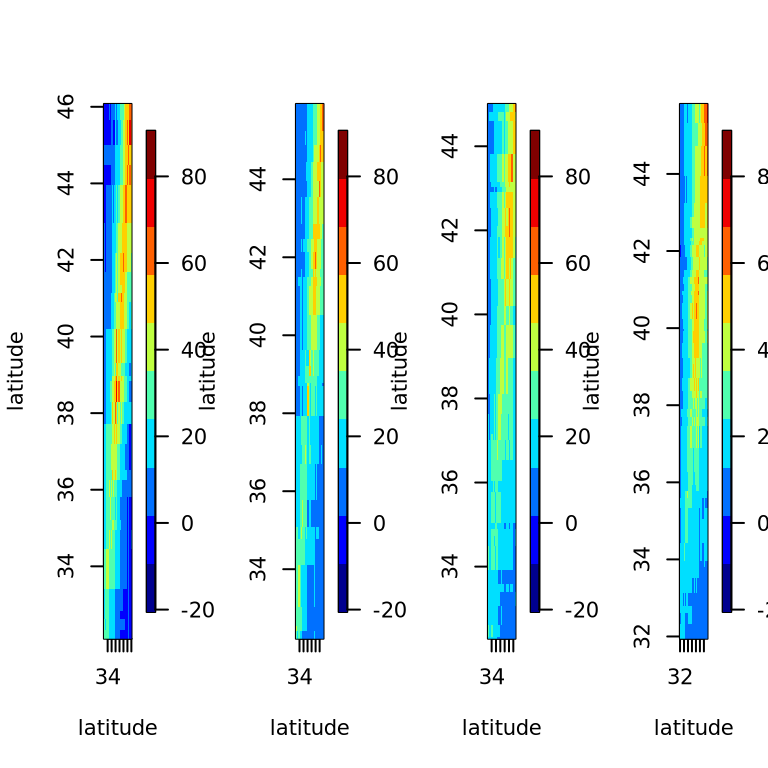
\includegraphics{note_stat501_files/figure-latex/unnamed-chunk-19-1} \end{center}

\hypertarget{compare-with-the-results-by-glm}{%
\paragraph{Compare with the results by
GLM}\label{compare-with-the-results-by-glm}}

Using glm function, the fitted logit model gives the largest value of
coefficients and residual scale.

Linear regression treat response as a continuous value {????} and gives
the smallest value of coefficients.

What is the benifit of log transform?

\begin{Shaded}
\begin{Highlighting}[]
\NormalTok{fit.probit.lm <-}\StringTok{ }\KeywordTok{lm}\NormalTok{(Resp}\OperatorTok{~}\NormalTok{Vol}\OperatorTok{+}\NormalTok{Rate)}
\NormalTok{fit.probit.glm <-}\StringTok{ }\KeywordTok{glm}\NormalTok{(Resp}\OperatorTok{~}\NormalTok{Vol}\OperatorTok{+}\NormalTok{Rate,}\DataTypeTok{family=}\KeywordTok{binomial}\NormalTok{(}\DataTypeTok{link=}\StringTok{"probit"}\NormalTok{))}
\NormalTok{fit.logit.glm <-}\StringTok{ }\KeywordTok{glm}\NormalTok{(Resp}\OperatorTok{~}\NormalTok{Vol}\OperatorTok{+}\NormalTok{Rate,}\DataTypeTok{family=}\KeywordTok{binomial}\NormalTok{(}\DataTypeTok{link=}\StringTok{"logit"}\NormalTok{))}
\NormalTok{comp <-}\StringTok{ }\KeywordTok{fits.compare}\NormalTok{(fit.probit.lm, fit.probit.glm, fit.logit.glm)}
\NormalTok{comp}
\CommentTok{## }
\CommentTok{## Calls: }
\CommentTok{## Name}
\CommentTok{## fit.probit.lm     lm(formula = Resp ~ Vol + Rate)}
\CommentTok{## fit.probit.glm    glm(formula = Resp ~ Vol + Rate, family = binomial(link = "probit"))}
\CommentTok{## fit.logit.glm     glm(formula = Resp ~ Vol + Rate, family = binomial(link = "logit"))}
\CommentTok{## }
\CommentTok{## }
\CommentTok{## Residual Statistics}
\CommentTok{##                   Min     1Q    Median    3Q   Max}
\CommentTok{## fit.probit.lm  -0.659 -0.365 0.0243305 0.266 0.797}
\CommentTok{## fit.probit.glm -0.699 -0.287 0.0000918 0.119 0.913}
\CommentTok{## fit.logit.glm  -0.687 -0.247 0.0012604 0.118 0.928}
\CommentTok{## }
\CommentTok{## }
\CommentTok{## Number of Parameter in each Model}
\CommentTok{##                Nobs Resid df Model Parameters Est. Parameters}
\CommentTok{## fit.probit.lm    39       36                3               3}
\CommentTok{## fit.probit.glm   39       36                3               3}
\CommentTok{## fit.logit.glm    39       36                3               3}
\CommentTok{## }
\CommentTok{## }
\CommentTok{## Coefficients:}
\CommentTok{##                            Estimate Std. Error t value}
\CommentTok{## (Intercept):fit.probit.lm  -0.610    0.220     -2.765 }
\CommentTok{## (Intercept):fit.probit.glm -5.060    1.512     -3.347 }
\CommentTok{## (Intercept):fit.logit.glm  -9.187    3.180     -2.889 }
\CommentTok{## Vol:fit.probit.lm           0.397    0.085      4.674 }
\CommentTok{## Vol:fit.probit.glm          2.022    0.665      3.041 }
\CommentTok{## Vol:fit.logit.glm           3.660    1.366      2.680 }
\CommentTok{## Rate:fit.probit.lm          0.343    0.080      4.299 }
\CommentTok{## Rate:fit.probit.glm         1.456    0.450      3.238 }
\CommentTok{## Rate:fit.logit.glm          2.593    0.928      2.794 }
\CommentTok{## }
\CommentTok{## }
\CommentTok{## Residual Scale Estimates:}
\CommentTok{## fit.probit.lm  : 0.389 on 36 degrees of freedom}
\CommentTok{## fit.probit.glm : 2.39 }
\CommentTok{## fit.logit.glm  : 11.5 }
\CommentTok{## }
\CommentTok{## Proportion of variation in response(s) explained by model(s):}
\CommentTok{## fit.probit.lm  : 0.442 }
\CommentTok{## }
\CommentTok{## F-statistics (NA if not available):}
\CommentTok{## fit.probit.lm  : 14.3 on 2 and 36 degrees of freedom, the  p-value is 0.0000273 }
\CommentTok{## }
\CommentTok{## Correlation of Coefficients:}
\CommentTok{## }
\CommentTok{## Model =  fit.probit.glm }
\CommentTok{##      (Intercept) Vol   }
\CommentTok{## Vol  -0.905            }
\CommentTok{## Rate -0.901       0.678}
\CommentTok{## }
\CommentTok{## Model =  fit.logit.glm  }
\CommentTok{##      (Intercept) Vol   }
\CommentTok{## Vol  -0.927            }
\CommentTok{## Rate -0.920       0.743}
\KeywordTok{plot}\NormalTok{(comp)}
\end{Highlighting}
\end{Shaded}

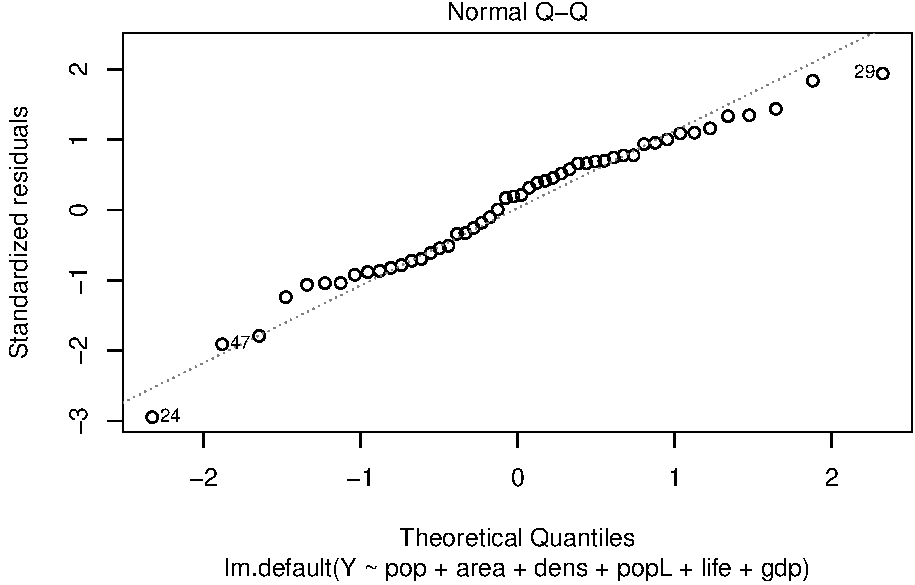
\includegraphics{note_stat501_files/figure-latex/unnamed-chunk-20-1.pdf}
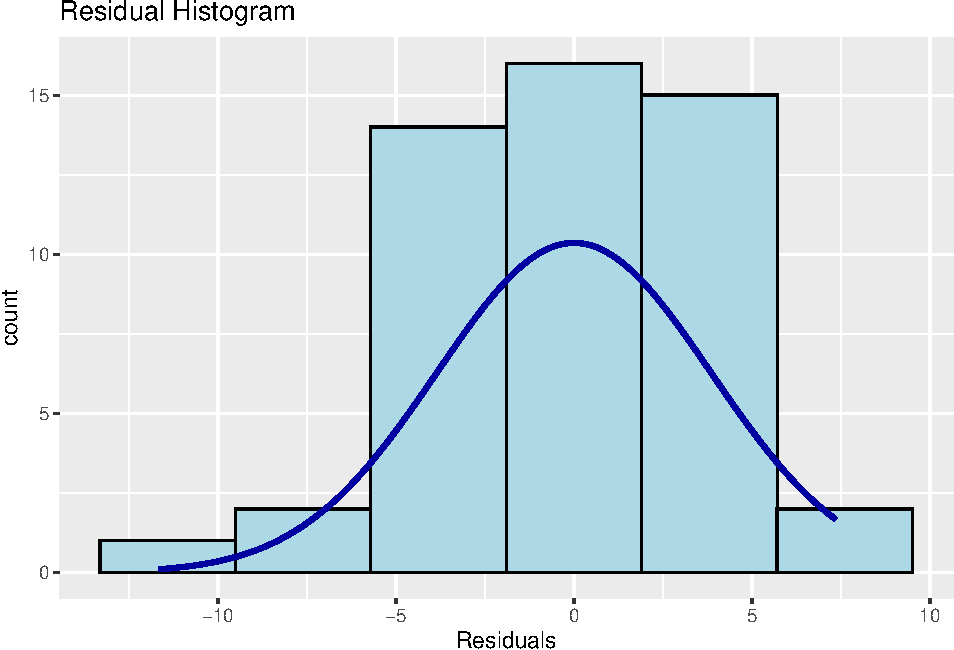
\includegraphics{note_stat501_files/figure-latex/unnamed-chunk-20-2.pdf}
\includegraphics{note_stat501_files/figure-latex/unnamed-chunk-20-3.pdf}

\hypertarget{compare-with-the-results-after-log-transform}{%
\paragraph{Compare with the results after log
transform}\label{compare-with-the-results-after-log-transform}}

\begin{Shaded}
\begin{Highlighting}[]
\NormalTok{fit.probit.lm.l <-}\StringTok{ }\KeywordTok{lm}\NormalTok{(Resp}\OperatorTok{~}\NormalTok{lVol}\OperatorTok{+}\NormalTok{lRate)}
\NormalTok{fit.probit.glm.l <-}\StringTok{ }\KeywordTok{glm}\NormalTok{(Resp}\OperatorTok{~}\NormalTok{lVol}\OperatorTok{+}\NormalTok{lRate,}\DataTypeTok{family=}\KeywordTok{binomial}\NormalTok{(}\DataTypeTok{link=}\StringTok{"probit"}\NormalTok{))}
\NormalTok{fit.logit.glm.l <-}\StringTok{ }\KeywordTok{glm}\NormalTok{(Resp}\OperatorTok{~}\NormalTok{lVol}\OperatorTok{+}\NormalTok{lRate,}\DataTypeTok{family=}\KeywordTok{binomial}\NormalTok{(}\DataTypeTok{link=}\StringTok{"logit"}\NormalTok{))}
\NormalTok{comp <-}\StringTok{ }\KeywordTok{fits.compare}\NormalTok{(fit.probit.lm.l, fit.probit.glm.l, fit.logit.glm.l)}
\NormalTok{comp}
\CommentTok{## }
\CommentTok{## Calls: }
\CommentTok{## Name}
\CommentTok{## fit.probit.lm.l     lm(formula = Resp ~ lVol + lRate)}
\CommentTok{## fit.probit.glm.l    glm(formula = Resp ~ lVol + lRate, family = binomial(link = "probit"))}
\CommentTok{## fit.logit.glm.l     glm(formula = Resp ~ lVol + lRate, family = binomial(link = "logit"))}
\CommentTok{## }
\CommentTok{## }
\CommentTok{## Residual Statistics}
\CommentTok{##                     Min     1Q  Median    3Q   Max}
\CommentTok{## fit.probit.lm.l  -0.625 -0.365 0.08625 0.295 0.739}
\CommentTok{## fit.probit.glm.l -0.663 -0.210 0.00127 0.169 0.907}
\CommentTok{## fit.logit.glm.l  -0.650 -0.168 0.00484 0.170 0.927}
\CommentTok{## }
\CommentTok{## }
\CommentTok{## Number of Parameter in each Model}
\CommentTok{##                  Nobs Resid df Model Parameters Est. Parameters}
\CommentTok{## fit.probit.lm.l    39       36                3               3}
\CommentTok{## fit.probit.glm.l   39       36                3               3}
\CommentTok{## fit.logit.glm.l    39       36                3               3}
\CommentTok{## }
\CommentTok{## }
\CommentTok{## Coefficients:}
\CommentTok{##                              Estimate Std. Error t value}
\CommentTok{## (Intercept):fit.probit.lm.l   0.231    0.081      2.844 }
\CommentTok{## (Intercept):fit.probit.glm.l -1.533    0.603     -2.543 }
\CommentTok{## (Intercept):fit.logit.glm.l  -2.924    1.267     -2.308 }
\CommentTok{## lVol:fit.probit.lm.l          0.595    0.125      4.759 }
\CommentTok{## lVol:fit.probit.glm.l         2.880    0.860      3.349 }
\CommentTok{## lVol:fit.logit.glm.l          5.220    1.827      2.857 }
\CommentTok{## lRate:fit.probit.lm.l         0.496    0.112      4.424 }
\CommentTok{## lRate:fit.probit.glm.l        2.556    0.836      3.059 }
\CommentTok{## lRate:fit.logit.glm.l         4.631    1.760      2.632 }
\CommentTok{## }
\CommentTok{## }
\CommentTok{## Residual Scale Estimates:}
\CommentTok{## fit.probit.lm.l  : 0.383 on 36 degrees of freedom}
\CommentTok{## fit.probit.glm.l : 2.01 }
\CommentTok{## fit.logit.glm.l  : 10 }
\CommentTok{## }
\CommentTok{## Proportion of variation in response(s) explained by model(s):}
\CommentTok{## fit.probit.lm.l  : 0.459 }
\CommentTok{## }
\CommentTok{## F-statistics (NA if not available):}
\CommentTok{## fit.probit.lm.l  : 15.3 on 2 and 36 degrees of freedom, the  p-value is 0.0000157 }
\CommentTok{## }
\CommentTok{## Correlation of Coefficients:}
\CommentTok{## }
\CommentTok{## Model =  fit.probit.glm.l }
\CommentTok{##       (Intercept) lVol  }
\CommentTok{## lVol  -0.754            }
\CommentTok{## lRate -0.908       0.753}
\CommentTok{## }
\CommentTok{## Model =  fit.logit.glm.l  }
\CommentTok{##       (Intercept) lVol  }
\CommentTok{## lVol  -0.809            }
\CommentTok{## lRate -0.929       0.805}
\CommentTok{# plot(comp)}
\end{Highlighting}
\end{Shaded}

\hypertarget{election-data}{%
\subsubsection{5.2 Election Data}\label{election-data}}

\hypertarget{a-trivariate-probit-example}{%
\subsubsection{5.3 A Trivariate Probit
Example}\label{a-trivariate-probit-example}}

\hypertarget{polson-etal-2013}{%
\subsection{(Polson etal, 2013)}\label{polson-etal-2013}}

Nicholas G. Polson, James G. Scott \& Jesse Windle (2013) Bayesian
Inference for Logistic Models Using Pólya--Gamma Latent Variables,
Journal of the American Statistical Association, 108:504, 1339-1349,
\href{https://www.tandfonline.com/doi/full/10.1080/01621459.2013.829001}{DOI:
10.1080/01621459.2013.829001}

\hypertarget{introduction-2}{%
\subsubsection{Introduction}\label{introduction-2}}

\href{https://jgscott.github.io/}{Home page of James Scott}

\href{https://github.com/jwindle/BayesLogit}{R package BayesLogit and
Thesis}

\emph{Definition 1}. A random variable X has a Pólya--Gamma distribution
with parameters b \textgreater{} 0 and , denoted as \(X\sim PG(b, c),\)
if

\[X\overset{\mathcal{D}}{=}\frac1{2\pi^2}\sum_{k=1}^\infty\frac{g_k}{((k-\frac12)^2 + \frac{c^2}{4\pi^2})}\quad (1)\]

where the \(g_k ∼ Ga(b, 1)\) are independent gamma random variables, and
where indicates equality in distribution.

\hypertarget{the-polya-gamma-distribution}{%
\subsubsection{2 The Polya-Gamma
distribution}\label{the-polya-gamma-distribution}}

\hypertarget{the-case-pgb0}{%
\paragraph{\texorpdfstring{2.1. The Case
\(PG(b,0)\)}{2.1. The Case PG(b,0)}}\label{the-case-pgb0}}

The \(PG(b,0)\) class of distributions is closely related to a subset of
distributions that are surveyed by Biane, Pitman, and Yor (2001). This
family of distributions, which we denote by \(J^\star(b), b>0\), has
close connections with {the Jacobi Theta and Riemann Zeta functions, and
with Brownian excursions}. Its Laplace transform is

\[E[\exp(-tJ^\star(b))]=\cosh^{-b}\sqrt{2t}\quad (4)\]

implying that \(PG(b,0)\overset{\mathcal{D}}{=}\frac14J^\star(b)\)

\hypertarget{the-general-pgbc-class}{%
\paragraph{\texorpdfstring{2.2. The General \(PG(b,c)\)
Class}{2.2. The General PG(b,c) Class}}\label{the-general-pgbc-class}}

\[p(x|b,c)=\frac{\exp(-\frac{c^2}2x) p(x|b,0)}{E[\exp x(-\frac{c^2}2\omega)]}\quad (5)\]

where \(p(x|b,0)\) is the density of an \(\omega\sim PG(b,0)\) random
variable.

\hypertarget{a-data-augmentation-strategy}{%
\subsubsection{3 A data-augmentation
strategy}\label{a-data-augmentation-strategy}}

A data-augmentation scheme for binomial likelihoods

\hypertarget{main-result}{%
\paragraph{3.1 Main Result}\label{main-result}}

\begin{longtable}[]{@{}lll@{}}
\toprule
& Polson et al.~(2013) & Albert and Chib (1993)\tabularnewline
\midrule
\endhead
Gaussian & scale mixture & location mixture\tabularnewline
Latent variables & Polya-Gamma & truncated normals\tabularnewline
\bottomrule
\end{longtable}

The number of successes
\(y_i\sim Bino(n_i,\frac{1}{\{1+e^{-\psi_i}\}})\), where \(n_i\) is the
number of trials, \(\psi_i=x_i^T\boldsymbol{\beta}\) are the log odds of
success. \(x_i=(x_{i1},..,x_{ip} )\) the vector of regressors for
observation \(i\in\{1,..,N\}\). \(\boldsymbol{\beta}\sim N(b,B)\)

To sample from the posterior distribution using the Pólya--Gamma method,
simply iterate two steps:

\[\begin{align}
(\omega_i|\boldsymbol{\beta})&\sim PG(n_i,x_i^T\boldsymbol{\beta})\\
(\boldsymbol{\beta}|y,\omega)&\sim N(m_\omega,V_\omega);\quad m_\omega=V_\omega(X^T\kappa+B^{-1}b);V_\omega=(X^T\Omega X+B^{-1})^{-1}
\end{align}\]

where \(\kappa=(y_1-\frac{n_1}2,..,y_N-\frac{n_N}2)\), and \(\Omega\) is
the diagonal matrix of \(\omega_i\)'s.

\hypertarget{existing-data-augmentation-schemes}{%
\paragraph{3.2 Existing Data-Augmentation
Schemes}\label{existing-data-augmentation-schemes}}

The outcomes \(y_i\) are assumed to be thresholded versions of an
underlying continuous quantity \(z_i\)

Assume \(n_i=1\),
\(y_i=\begin{cases}1&\text{if } z_i>0\\0&\text{if }z_i\le0\end{cases}\)

\(z_i=x_i^T\boldsymbol{\beta}+\epsilon_i\),
\(\epsilon_i\sim Logistic(1)\)

The standard approach has been to add another layer of auxiliary
variables to handle the logistic error model on the latent-utility
scale. One strategy is to represent the logistic distribution as a
normal-scale mixture

\[(\epsilon_i|\phi_i)\sim N(0,\phi_i);\quad \phi_i=(2\lambda_i)^2; \lambda_i\sim KS(1)\quad\text{Kolmogorov–Smirnov distribution}\]

Alternatively, one may approximate the logistic error term as a discrete
mixture of normals.

\[(\epsilon_i|\phi_i)\sim N(0,\phi_i);\quad \phi_i=\sum_{k=1}^K\omega_k\delta_{\phi^{(k)}}\]

where \(\delta_{\phi}\) indicates a {\emph{Dirac measure}} at \(\phi\).
The weights \(\omega_k\) and the points \(\phi^{(k)}\) in the discrete
mixture are fixed for a given choice of \(k\) so that \emph{{the
Kullback--Leibler divergence}} from the true distribution of the random
utilities is minimized. Frühwirth-Schnatter and Frühwirth (2010) found
that the choice of \(K=10\) leads to a good approximation.

The discrete mixture of normals is an approximation, but it outperforms
the scale mixture of normals in terms of effective sampling rate, as it
is much faster.

One may also arrive at the hierarchy above by manipulating the random
utility derivation of McFadden (1974)

The dRUM. One must use a table of different weights and variances
representing different normal mixtures, to approximate a finite
collection of type-III logistic distributions, and interpolate within
this table to approximate the entire family.

Another approximation: the use of a Student-t link function as a close
substitute for the logistic link. This also introduces a second layer of
latent variables, in that the Student-t error model for \(z_i\) is
represented as a scale mixture of normals.

Our data-augmentation scheme differs from each of these approaches in
several ways.

\begin{enumerate}
\def\labelenumi{\arabic{enumi}.}
\item
  it does not appeal directly to the random-utility interpretation of
  the logit model. Instead, it represents the logistic CDF as a mixture
  with respect to an infinite convolution of gammas.
\item
  the method is exact, in the sense of making draws from the correct
  joint posterior distribution, rather than an approximation to the
  posterior that arises out of an approximation to the link function.
\item
  like the Albert and Chib (1993) method, it requires only a single
  layer of latent variables.
\end{enumerate}

Directed acyclic graphs depicting two latent-variable constructions for
the logistic-regression model: the difference of random-utility model
versus direct data-augmentation scheme.
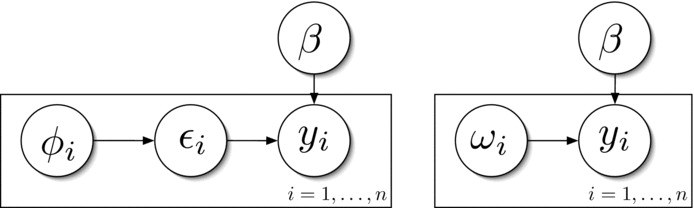
\includegraphics{uasa_a_829001_o_f0001g.jpeg}

\hypertarget{mixed-model-example}{%
\paragraph{3.3. Mixed Model Example}\label{mixed-model-example}}

The real advantage of data augmentation, and the Pólya--Gamma technique
in particular, is that it becomes easy to construct and fit more
complicated models. For instance, the Pólya--Gamma method trivially
accommodates \emph{mixed models, factor models, and models with a
spatial or dynamic structure}. For most problems in this class, good MH
samplers are difficult to design, and at the very least will require ad
hoc tuning to yield good performance.

\[\begin{align}
y_{ij}&\sim Bino(1,p_{ij}),\quad p_{ij}=\frac{e^{\psi_{ij}}}{1+e^{\psi_{ij}}}\\
\psi_{ij}&=m+\delta_j+x'_{ij}\beta,\quad\delta_j\sim N(0,1/\phi);\quad m\sim N(0,\kappa^2/\phi)
\end{align}\]

where \(i\) and \(j\) correspond to the \(i^{th}\) observation from the
\(j^{th}\) district. The fixed effect \(\beta\) is given an
\(N(0, 100I)\) prior, while the precision parameter \(\phi\) is given
\(Ga(1, 1)\) prior. We take \(\kappa\to\infty\) to recover an improper
prior for the global intercept \(m\).

Bangladesh Fertility Survey, 1989

\begin{Shaded}
\begin{Highlighting}[]
\KeywordTok{data}\NormalTok{(Contraception)}
\end{Highlighting}
\end{Shaded}

As seen in the negative binomial examples below, one may also painlessly
incorporate a more complex prior structure using the Pólya--Gamma
technique. For instance, if given information about \emph{the geographic
location} of each district, one could place a \emph{spatial process
prior} upon the random offsets \(\{\delta_j\}\).

\hypertarget{simulating-polya-gamma-random-variables}{%
\subsubsection{4 Simulating Polya-Gamma random
Variables}\label{simulating-polya-gamma-random-variables}}

a method for simulating from the Pólya--Gamma distribution, which we
have implemented as a stand-alone sampler in the BayesLogit R package.

\hypertarget{the-pg1z-sampler}{%
\paragraph{\texorpdfstring{4.1. The \(PG(1,z)\)
Sampler}{4.1. The PG(1,z) Sampler}}\label{the-pg1z-sampler}}

An exponentially tilted Jacobi distribution \(J^\star(1,z)\) via the
density

\[f(x|z)=\cosh(z)\exp\left(-\frac{z^{2}x}2\right)f(x)\quad(9)\]
\[PG(1,z)=\frac14J^\star(1,\frac z2)\quad (10)\]

When \(f(x)=\sum_{n=0}^\infty(-1)^na_n(x)\) and the coefficients
\(a_n(x)\) are decreasing for all , for fixed \(x\) in the support of
\(f\), then the partial sums, \(S_n(x)=\sum_{i=0}^n(-1)^ia_i(x)\),
satisfy

\[S_0(x)>S_2(x)>..>f(x)>..>S_3(x)>S_1(x)\quad (11)\]

For the \(J^\star(1,z)\) distribution the algorithm will accept with
high probability upon checking \(U\le S_1(X)\).

The Jacobi density has two alternating-sum representations,
\(\sum_{n=0}^\infty(-1)^na_i^L(x)\) and
\(\sum_{n=0}^\infty(-1)^na_i^R(x)\), neither of which satisfy Equation
(11) for all \(x\) in the support of \(f\). However, each satisfies
Equation (11) on an interval. These two intervals, respectively, denoted
as \(I_L\) and \(I_R\) , satisfy \(I_L\cup I_R = (0,\infty)\) and
\(I_L\cap I_R\neq\emptyset\) Thus, one may pick \(t\in I_L\cap I_R\)and
define the piecewise coefficients.

\[a_n(x)=\pi(n+\frac{1}2)\begin{cases}(\frac{2}{\pi x})^{\frac32}\exp\left(-\frac{2(n+\frac{1}2)^2}{x}\right) & 0<x\le t&(12)\\ \exp\left(-(\frac{\pi^2(n+\frac{1}2)^{2}}2)x\right) & x>t&(13)\end{cases}\]

so that \(f(x)=\sum_{n=0}^\infty(-1)^na_n(x)\) satisfies the partial sum
criterion (11) for \(x>0\). Devroye shows that the best choice of \(t\)
is near 0.64.

The \(J^\star(1,z)\) density can be written as an infinite, alternating
sum \(f(x|z)=\sum_{n=0}^\infty(-1)^na_n(x|z)\), where

\[a_n(x|z)=\cosh(z)\exp\left(-\frac{z^{2}x}2\right)a_n(x)\]

This satisfies Equation (11), as
\(\frac{a_{n+1}(x|z)}{a_n(x|z)}=\frac{a_{n+1}(x)}{a_n(x)}\).

Since \(a_0(x|z)\ge f(x|z)\), the first term of the series provides a
natural proposal:

\[c(z) g(x|z)=\frac{\pi}2\cosh(z)\begin{cases}(\frac{2}{\pi x})^{\frac32}\exp\left(-\frac{z^{2}x}2-\frac{1}{2x}\right) & 0<x\le t\\ \exp\left(-(\frac{z^{2}}2+\frac{\pi^{2}}8)x\right) & x>t\end{cases}(14)\]

\(X\sim g(x|z)\) may be sampled from a mixture of an inverse-Gaussian
and an exponential:

\[X\sim \begin{cases}IG(|z|^{-1},1)\mathbf{1}_{(0,t]} & \text{with prob } \frac{p}{p+q}\\ Expo(-\frac{z^{2}}2+\frac{\pi^{2}}8)\mathbf{1}_{(t,\infty)} & \text{with prob } \frac{q}{p+q}\end{cases}\]

where \(p(z) =\int^t_0 c(z) g(x|z)dx\) and
\(q(z) =\int_t^\infty c(z) g(x|z)dx\). Note that we are implicitly
suppressing the dependence of p, q, c, and g upon t.

{\(Expo(-(\frac{z^{2}}2+\frac{\pi^{2}}8))\)???}

sampling \(J^\star(1,z)\) proceeds as follows:

\begin{enumerate}
\def\labelenumi{\arabic{enumi}.}
\item
  Generate a proposal \(X\sim g(x|z)\).
\item
  Generate \(U\sim Unif(0,c(z)g(X|z))\).
\item
  Iteratively calculate \(S_n (X|z)\), starting at \(S_1(X|z)\), until
  \(U\le S_n(X|z)\) for an odd \(n\) or until \(U>S_n (X|z)\) for an
  even \(n\).
\item
  Accept \(X\) if \(n\) is odd; return to step 1 if \(n\) is even.
\end{enumerate}

To sample \(Y\sim PG(1, z)\), draw \(X\sim J^\star(1,z/2)\) and then let
\(Y=X/4\)

\hypertarget{analysis-of-acceptance-rate}{%
\paragraph{4.2. Analysis of Acceptance
Rate}\label{analysis-of-acceptance-rate}}

\textbf{Proposition 1} Define

\[p(z,t)=\int^t_0 \frac\pi2\cosh(z)\exp\left(-\frac{z^{2}x}2\right)a_0^L(x)dx\]
\[q(z,t)=\int^\infty_t \frac\pi2\cosh(z)\exp\left(-\frac{z^{2}x}2\right)a_0^R(x)dx\]

\begin{enumerate}
\def\labelenumi{\arabic{enumi}.}
\item
  The best truncation point \(t^\star\) is independent of \(z\ge0\).
\item
  For a fixed truncation point \(t\), \(p(z,t)\) and \(q(z,t)\) are
  continuous, \(p(z,t)\) decreases to zero as \(z\) diverges, and
  \(q(z, t)\) converges to 1 as \(z\) diverges. Thus,
  \(c(z,t)= p(z,t) + q(z,t)\) is continuous and converges to 1 as \(z\)
  diverges.
\item
  For fixed \(t\), the average probability of accepting a draw,
  \(1/c(z,t)\), is bounded below for all \(z\). For \(t^\star\), this
  bound to five digits is \(0.99919\), which is attained at
  \(z\simeq1.378.\)
\end{enumerate}

\hypertarget{analysis-of-tail-probabilities}{%
\paragraph{4.3. Analysis of Tail
Probabilities}\label{analysis-of-tail-probabilities}}

\textbf{Proposition 2}: When sampling \(X\sim J^\star(1, z)\), the
probability of deciding to accept or reject upon checking the \(n^{th}\)
partial sum \(S_n\), \(n\ge1\), is

\[\frac1{c(z)}\int^\infty_0 [a_{n-1}(x|z)-a_n(x|z)]dx\]

\hypertarget{the-general-pgb-z-case}{%
\paragraph{\texorpdfstring{4.4. The General \(PG(b, z)\)
Case}{4.4. The General PG(b, z) Case}}\label{the-general-pgb-z-case}}

The effective sample size (ESS) for the ith parameter in the model is

\[ESS_i=\frac{M}{1+2\sum_{j=1}^k\rho_i(j)}\]

where \(M\) is the number of post-burn-in samples, and \(\rho_i(j)\) is
the \(j^{th}\) autocorrelation of the chain corresponding to \(\beta_i\)

\hypertarget{experiment}{%
\subsubsection{5 Experiment}\label{experiment}}

presents the results of an extensive benchmarking study comparing the
efficiency of our method to other data-augmentation schemes.

The eight datasets

\begin{itemize}
\tightlist
\item
  In binary logit models.
\end{itemize}

First, the Pólya--Gamma is more efficient than all previously proposed
data-augmentation schemes.

Second, the Pólya--Gamma method always had a higher effective sample
size than the two default Metropolis samplers we tried.

Finally, the Pólya--Gamma method truly shines when the model has a
complex prior structure.

\begin{itemize}
\tightlist
\item
  In negative-binomial models.
\end{itemize}

The Pólya--Gamma method consistently yields the best effective sample
sizes in negative-binomial regression. However, its effective sampling
rate suffers when working with a large count or a nonintegral
overdispersion parameter.

Using either the Pólya--Gamma or the Frühwirth-Schnatter et al.~(2009)
techniques, one arrives at a multivariate Gaussian conditional for
\(\psi\) whose covariance matrix involves latent variables. Producing a
random variate from this distribution is expensive, as one must
calculate the Cholesky decomposition of a relatively large matrix at
each iteration. Therefore, the overall sampler spends relatively less
time drawing auxiliary variables. Since the Pólya--Gamma method leads to
a higher effective sample size, it wastes fewer of the expensive draws
for the main parameter.

\hypertarget{discussion}{%
\subsubsection{6 Discussion}\label{discussion}}

concludes with a discussion of some open issues related to our proposal.

\hypertarget{technical-supplement}{%
\subsubsection{Technical supplement}\label{technical-supplement}}

\hypertarget{details-of-polya-gamma-sampling-algorithm}{%
\paragraph{1 Details of Polya-Gamma sampling
algorithm}\label{details-of-polya-gamma-sampling-algorithm}}

\hypertarget{benchmarks-overview}{%
\paragraph{2 Benchmarks: overview}\label{benchmarks-overview}}

\hypertarget{benchmarks-binary-logistic-regression}{%
\paragraph{3 Benchmarks: binary logistic
regression}\label{benchmarks-binary-logistic-regression}}

\hypertarget{data-sets}{%
\subparagraph{3.1 Data Sets}\label{data-sets}}

Nodal: part of the boot R package (Canty and Ripley, 2012). The response
indicates if cancer has spread from the prostate to surrounding lymph
nodes. There are 53 observations and 5 binary predictors.

Pima Indian: There are 768 observations and 8 continuous predictors. It
is noted on
\href{http://archive.ics.uci.edu/ml/datasets/Pima+Indians+Diabetes}{the
UCI website} that there are many predictor values coded as 0, though the
physical measurement should be non-zero. We have removed all of those
entries to generate a data set with 392 observations. The marginal mean
incidence of diabetes is roughly 0.33 before and after removing these
data points.

\href{http://archive.ics.uci.edu/ml/datasets/Statlog+(Heart)}{Heart}:
The response represents either an absence or presence of heart disease.
There are 270 observations and 13 attributes, of which 6 are categorical
or binary and 1 is ordinal. The ordinal covariate has been stratified by
dummy variables.

\href{http://archive.ics.uci.edu/ml/datasets/Statlog+(Australian+Credit+Approval)}{Australian
Credit}: The response represents either accepting or rejecting a credit
card application.3 The meaning of each predictor was removed to protect
the propriety of the original data. There are 690 observations and 14
attributes, of which 8 are categorical or binary. There were 37
observations with missing attribute values. These missing values were
replaced by the mode of the attribute in the case of categorical data
and the mean of the attribute for continuous data. This dataset is
linearly separable and results in some divergent regression
coefficients, which are kept in check by the prior.

\href{http://archive.ics.uci.edu/ml/datasets/Statlog+(German+Credit+Data)}{German
Credit 1 and 2}: The response represents either a good or bad credit
risk.4 There are 1000 observations and 20 attributes, including both
continuous and categorical data. We benchmark two scenarios. In the
first, the ordinal covariates have been given integer values and have
not been stratified by dummy variables, yielding a total of 24 numeric
predictors. In the second, the ordinal data has been stratified by dummy
variables, yielding a total of 48 predictors.

Synthetic 1: Simulated data with 150 outcomes and 10 predictors. The
design points were chosen to be orthogonal. The data are included as a
supplemental file.

Synthetic 2: Simulated data with 500 outcomes and 20 predictors. The
design points were simulated from a Gaussian factor model, to yield
pronounced patterns of collinearity. The data are included as a
supplemental file.

\hypertarget{methods}{%
\subparagraph{3.2 Methods}\label{methods}}

\hypertarget{results}{%
\subparagraph{3.3 Results}\label{results}}

\hypertarget{benchmarks-logit-mixed-models}{%
\paragraph{4 Benchmarks: logit mixed
models}\label{benchmarks-logit-mixed-models}}

\hypertarget{benchmarks-negative-binomial-models}{%
\paragraph{5 Benchmarks: negative-binomial
models}\label{benchmarks-negative-binomial-models}}

\hypertarget{extensions}{%
\paragraph{6 Extensions}\label{extensions}}

\hypertarget{choi-hobert-2013}{%
\subsection{(Choi \& Hobert, 2013)}\label{choi-hobert-2013}}

Choi, H. M., \& Hobert, J. P. (2013). The Polya-Gamma Gibbs sampler for
Bayesian logistic regression is uniformly ergodic.
\href{https://projecteuclid.org/euclid.ejs/1377005819}{Electronic
Journal of Statistics, 7, 2054-2064.}

\hypertarget{introduction-3}{%
\paragraph{1 Introduction}\label{introduction-3}}

\hypertarget{polson-scott-and-windles-algorithm}{%
\paragraph{2 Polson, Scott and Windle's
algorithm}\label{polson-scott-and-windles-algorithm}}

\hypertarget{taylor-rodruxedguez-et-al-2017}{%
\subsection{(Taylor-Rodríguez et al,
2017)}\label{taylor-rodruxedguez-et-al-2017}}

Taylor-Rodríguez, D., Womack, A., Fuentes, C., \& Bliznyuk, N. (2017).
Intrinsic Bayesian Analysis for Occupancy Models.
\href{https://projecteuclid.org/euclid.ba/1473431536}{Bayesian Anal.,
12(3), 855-877.}

\hypertarget{introduction-4}{%
\subsubsection{1 Introduction}\label{introduction-4}}

\hypertarget{inference-for-a-single-model}{%
\subsubsection{2 Inference for a single
model}\label{inference-for-a-single-model}}

\hypertarget{the-occupancy-model-with-probit-link}{%
\paragraph{2.1 The occupancy model with Probit
link}\label{the-occupancy-model-with-probit-link}}

\hypertarget{an-objective-prior-for-ux3b1-ux3bb}{%
\paragraph{2.2 An objective prior for (α,
λ)}\label{an-objective-prior-for-ux3b1-ux3bb}}

\hypertarget{resources}{%
\subsection{Resources}\label{resources}}

\href{http://users.stat.umn.edu/~geyer/}{Charlie Geyer's Personal Home
Page}

\href{https://xcelab.net/rm/statistical-rethinking/}{McElreath 2020.
Statistical Rethinking}

\href{https://github.com/rmcelreath/rethinking}{R package rethinking}

\end{document}
